\documentclass[11pt,a4paper]{article}

\usepackage[T1]{fontenc}
\usepackage[utf8]{inputenc}
\usepackage{lmodern}
\usepackage[french]{babel}
\usepackage[a4paper,margin=2.5cm]{geometry}
\usepackage{amsmath,amssymb,amsthm,mathtools}
\usepackage{bm}
\usepackage{graphicx}
\usepackage{booktabs}
\usepackage{array}
\usepackage{enumitem}
\usepackage{xcolor}
\usepackage[ruled,vlined,linesnumbered,french]{algorithm2e}
\usepackage{microtype}
\usepackage[hidelinks]{hyperref}
\usepackage[nameinlink,noabbrev]{cleveref}
\usepackage{caption}
\usepackage{subcaption}
\setlength{\emergencystretch}{3em}
\usepackage[section]{placeins}

\graphicspath{{../results/figures/}}

% ---------------- Théorèmes ----------------
\theoremstyle{plain}
\newtheorem{theoreme}{Théorème}[section]
\newtheorem{proposition}[theoreme]{Proposition}
\newtheorem{lemme}[theoreme]{Lemme}
\newtheorem{corollaire}[theoreme]{Corollaire}
\theoremstyle{definition}
\newtheorem{definition}[theoreme]{Définition}
\newtheorem{exemple}[theoreme]{Exemple}
\newtheorem{hypothese}[theoreme]{Hypothèse}
\theoremstyle{remark}
\newtheorem{remarque}[theoreme]{Remarque}

\crefname{theoreme}{théorème}{théorèmes}
\crefname{proposition}{proposition}{propositions}
\crefname{lemme}{lemme}{lemmes}
\crefname{corollaire}{corollaire}{corollaires}
\crefname{definition}{définition}{définitions}
\crefname{remarque}{remarque}{remarques}
\crefname{figure}{figure}{figures}
\crefname{table}{tableau}{tableaux}
\crefname{section}{section}{sections}
\crefname{equation}{équation}{équations}

% ---------------- Notations ----------------
\newcommand{\R}{\mathbb{R}}
\newcommand{\N}{\mathbb{N}}
\newcommand{\E}{\mathbb{E}}
\renewcommand{\P}{\mathbb{P}}
\newcommand{\cS}{\mathcal{S}}
\newcommand{\cA}{\mathcal{A}}
\newcommand{\cM}{\mathcal{M}}
\newcommand{\cF}{\mathcal{F}}
\newcommand{\norm}[1]{\left\lVert #1 \right\rVert}
\newcommand{\ninf}[1]{\left\lVert #1 \right\rVert_\infty}
\newcommand{\abs}[1]{\left\lvert #1 \right\rvert}
\newcommand{\Rmax}{R_{\max}}
\newcommand{\1}{\mathbf{1}}
\DeclareMathOperator*{\argmax}{arg\,max}

\newcolumntype{C}{>{\centering\arraybackslash}p{1.6cm}}

% Fichier généré automatiquement par report/make_results.py. Ne pas éditer.
\newcommand{\MarkovPtwo}{\ensuremath{\begin{pmatrix}0.33 & 0.36 & 0.24 & 0.07\\0.22 & 0.39 & 0.25 & 0.14\\0.15 & 0.34 & 0.30 & 0.21\\0.07 & 0.29 & 0.31 & 0.33\end{pmatrix}}}
\newcommand{\MarkovPthree}{\ensuremath{\begin{pmatrix}0.261 & 0.365 & 0.255 & 0.119\\0.213 & 0.364 & 0.264 & 0.159\\0.173 & 0.347 & 0.281 & 0.199\\0.124 & 0.325 & 0.295 & 0.256\end{pmatrix}}}
\newcommand{\MarkovPtwoOneFour}{\ensuremath{0.07}}
\newcommand{\MarkovRuns}{\ensuremath{100\,000}}
\newcommand{\MarkovMC}{\ensuremath{(0.2633,\ 0.3642,\ 0.2550,\ 0.1175)}}
\newcommand{\MarkovExactRow}{\ensuremath{(0.261,\ 0.365,\ 0.255,\ 0.119)}}
\newcommand{\MarkovDev}{\ensuremath{0.0023}}
\newcommand{\MarkovStd}{\ensuremath{0.0016}}
\newcommand{\MarkovMu}{\ensuremath{(0.1955,\ 0.3526,\ 0.2724,\ 0.1795)}}
\newcommand{\ContrMaxNine}{\ensuremath{0.9000}}
\newcommand{\ContrEqNine}{\ensuremath{0.9000}}
\newcommand{\ContrMeanNine}{\ensuremath{0.458}}
\newcommand{\NumGreedyMatch}{\ensuremath{6.0\times10^{-14}}}
\newcommand{\NumRandomPolicies}{\ensuremath{20\,000}}
\newcommand{\NumMaxQpiMinusQstar}{\ensuremath{2.8\times10^{-14}}}
\newcommand{\NumBestRandom}{\ensuremath{-4.501}}
\newcommand{\VstarS}{\ensuremath{-2.483}}
\newcommand{\ActionGap}{\ensuremath{0.188}}
\newcommand{\ActionGapHalf}{\ensuremath{0.094}}
\newcommand{\VIRatioLast}{\ensuremath{0.4975}}
\newcommand{\SpectralRho}{\ensuremath{0.5528}}
\newcommand{\AsymptoticRate}{\ensuremath{0.4975}}
\newcommand{\VIIters}{\ensuremath{35}}
\newcommand{\VIBoundIters}{\ensuremath{196}}
\newcommand{\VIAPost}{\ensuremath{7.8\times10^{-8}}}
\newcommand{\VITrueErr}{\ensuremath{8.6\times10^{-9}}}
\newcommand{\VILastInc}{\ensuremath{8.7\times10^{-9}}}
\newcommand{\VIErrZero}{\ensuremath{8.537}}
\newcommand{\QstarSup}{\ensuremath{8.537}}
\newcommand{\ReturnBound}{\ensuremath{100}}
\newcommand{\LossEpsSmall}{\ensuremath{0.000}}
\newcommand{\LossEpsOne}{\ensuremath{0.229}}
\newcommand{\LossBoundOne}{\ensuremath{20}}
\newcommand{\LossEpsTwo}{\ensuremath{15.17}}
\newcommand{\LossBoundTwo}{\ensuremath{40}}
\newcommand{\MainAErrFinal}{\ensuremath{2.06}}
\newcommand{\MainAErrFinalMedian}{\ensuremath{0.26}}
\newcommand{\MainAErrThousand}{\ensuremath{7.32}}
\newcommand{\MainAErrTenK}{\ensuremath{4.07}}
\newcommand{\MainAErrFiftyK}{\ensuremath{2.97}}
\newcommand{\MainAErrHundred}{\ensuremath{9.72}}
\newcommand{\MainAMeanErrFinal}{\ensuremath{0.450}}
\newcommand{\MainAStartErrFinal}{\ensuremath{0.419}}
\newcommand{\MainAFracOpt}{\ensuremath{95.8\,\%}}
\newcommand{\MainAGreedyValue}{\ensuremath{-2.520}}
\newcommand{\MainAStab}{\ensuremath{17}}
\newcommand{\MainAStabMedian}{\ensuremath{22\,450}}
\newcommand{\MainASlope}{\ensuremath{-0.28}}
\newcommand{\MainASlopeMean}{\ensuremath{-0.34}}
\newcommand{\MainAVisitsMin}{\ensuremath{243}}
\newcommand{\MainAVisitsMax}{\ensuremath{85\,765}}
\newcommand{\MainAVisitsRatio}{\ensuremath{353}}
\newcommand{\MainACorr}{\ensuremath{-0.53}}
\newcommand{\MainAErrMax}{\ensuremath{16.81}}
\newcommand{\MainAErrMin}{\ensuremath{0.18}}
\newcommand{\MainAAvgReturn}{\ensuremath{-2.61}}
\newcommand{\MainAAvgLength}{\ensuremath{8.53}}
\newcommand{\MainANSeeds}{\ensuremath{20}}
\newcommand{\MainBErrFinal}{\ensuremath{0.28}}
\newcommand{\MainBErrFinalMedian}{\ensuremath{0.27}}
\newcommand{\MainBErrThousand}{\ensuremath{3.90}}
\newcommand{\MainBErrTenK}{\ensuremath{1.23}}
\newcommand{\MainBErrFiftyK}{\ensuremath{0.35}}
\newcommand{\MainBErrHundred}{\ensuremath{7.10}}
\newcommand{\MainBMeanErrFinal}{\ensuremath{0.057}}
\newcommand{\MainBStartErrFinal}{\ensuremath{0.205}}
\newcommand{\MainBFracOpt}{\ensuremath{100.0\,\%}}
\newcommand{\MainBGreedyValue}{\ensuremath{-2.483}}
\newcommand{\MainBStab}{\ensuremath{20}}
\newcommand{\MainBStabMedian}{\ensuremath{12\,025}}
\newcommand{\MainBSlope}{\ensuremath{-0.65}}
\newcommand{\MainBSlopeMean}{\ensuremath{-0.56}}
\newcommand{\MainBVisitsMin}{\ensuremath{256}}
\newcommand{\MainBVisitsMax}{\ensuremath{62\,142}}
\newcommand{\MainBVisitsRatio}{\ensuremath{243}}
\newcommand{\MainBCorr}{\ensuremath{-0.29}}
\newcommand{\MainBErrMax}{\ensuremath{0.52}}
\newcommand{\MainBErrMin}{\ensuremath{0.16}}
\newcommand{\MainBAvgReturn}{\ensuremath{3.33}}
\newcommand{\MainBAvgLength}{\ensuremath{4.79}}
\newcommand{\MainBNSeeds}{\ensuremath{20}}
\newcommand{\MainAArgmaxFar}{\ensuremath{13}}
\newcommand{\GammaVIItersLow}{\ensuremath{20}}
\newcommand{\GammaVIItersHigh}{\ensuremath{41}}
\newcommand{\GammaBoundHigh}{\ensuremath{2\,049}}
\newcommand{\GammaRelMin}{\ensuremath{3.9\,\%}}
\newcommand{\GammaRelMax}{\ensuremath{4.6\,\%}}
\newcommand{\GammaBoundLow}{\ensuremath{30}}
\newcommand{\GammaStabHighest}{\ensuremath{16\,025}}
\newcommand{\GammaRelThousandLow}{\ensuremath{27\,\%}}
\newcommand{\GammaRelThousandHigh}{\ensuremath{63\,\%}}
\newcommand{\GammaStabLow}{\ensuremath{5\,300}}
\newcommand{\GammaStabHigh}{\ensuremath{23\,450}}
\newcommand{\AlphaOneFinal}{\ensuremath{1.27}}
\newcommand{\AlphaOneTenK}{\ensuremath{1.65}}
\newcommand{\AlphaOneThousand}{\ensuremath{2.61}}
\newcommand{\AlphaOneStd}{\ensuremath{0.35}}
\newcommand{\AlphaOneMeanFinal}{\ensuremath{0.379}}
\newcommand{\AlphaOneTailMin}{\ensuremath{0.81}}
\newcommand{\AlphaOneTailMax}{\ensuremath{3.40}}
\newcommand{\AlphaFiveFinal}{\ensuremath{7.90}}
\newcommand{\AlphaFiveTenK}{\ensuremath{6.35}}
\newcommand{\AlphaFiveThousand}{\ensuremath{6.70}}
\newcommand{\AlphaFiveStd}{\ensuremath{1.73}}
\newcommand{\AlphaFiveMeanFinal}{\ensuremath{2.015}}
\newcommand{\AlphaFiveTailMin}{\ensuremath{3.38}}
\newcommand{\AlphaFiveTailMax}{\ensuremath{13.50}}
\newcommand{\AlphaNineFinal}{\ensuremath{12.62}}
\newcommand{\AlphaNineTenK}{\ensuremath{13.36}}
\newcommand{\AlphaNineThousand}{\ensuremath{12.77}}
\newcommand{\AlphaNineStd}{\ensuremath{2.26}}
\newcommand{\AlphaNineMeanFinal}{\ensuremath{4.333}}
\newcommand{\AlphaNineTailMin}{\ensuremath{7.27}}
\newcommand{\AlphaNineTailMax}{\ensuremath{21.41}}
\newcommand{\AlphaInvFinal}{\ensuremath{1.61}}
\newcommand{\AlphaInvTenK}{\ensuremath{2.74}}
\newcommand{\AlphaInvThousand}{\ensuremath{4.55}}
\newcommand{\AlphaInvStd}{\ensuremath{0.14}}
\newcommand{\AlphaInvMeanFinal}{\ensuremath{0.506}}
\newcommand{\AlphaInvTailMin}{\ensuremath{1.60}}
\newcommand{\AlphaInvTailMax}{\ensuremath{2.09}}
\newcommand{\AlphaPolyFinal}{\ensuremath{0.35}}
\newcommand{\AlphaPolyTenK}{\ensuremath{1.17}}
\newcommand{\AlphaPolyThousand}{\ensuremath{4.09}}
\newcommand{\AlphaPolyStd}{\ensuremath{0.09}}
\newcommand{\AlphaPolyMeanFinal}{\ensuremath{0.080}}
\newcommand{\AlphaPolyTailMin}{\ensuremath{0.29}}
\newcommand{\AlphaPolyTailMax}{\ensuremath{0.66}}
\newcommand{\ScMean}{\ensuremath{7.40}}
\newcommand{\ScVar}{\ensuremath{27.84}}
\newcommand{\ScN}{\ensuremath{20\,000}}
\newcommand{\ScRuns}{\ensuremath{200}}
\newcommand{\ScTheoOne}{\ensuremath{1.465}}
\newcommand{\ScTheoFive}{\ensuremath{9.28}}
\newcommand{\ScTheoInv}{\ensuremath{1.39\times10^{-3}}}
\newcommand{\ScFiveMSE}{\ensuremath{8.780}}
\newcommand{\ScFiveTail}{\ensuremath{9.281}}
\newcommand{\ScFiveMean}{\ensuremath{7.659}}
\newcommand{\ScOneMSE}{\ensuremath{1.279}}
\newcommand{\ScOneTail}{\ensuremath{1.465}}
\newcommand{\ScOneMean}{\ensuremath{7.341}}
\newcommand{\ScInvMSE}{\ensuremath{1.48\times10^{-3}}}
\newcommand{\ScInvTail}{\ensuremath{2.20\times10^{-3}}}
\newcommand{\ScInvMean}{\ensuremath{7.402}}
\newcommand{\ScPolyMSE}{\ensuremath{6.72\times10^{-3}}}
\newcommand{\ScPolyTail}{\ensuremath{7.04\times10^{-3}}}
\newcommand{\ScPolyMean}{\ensuremath{7.396}}
\newcommand{\ScSqMSE}{\ensuremath{8.596}}
\newcommand{\ScSqTail}{\ensuremath{8.596}}
\newcommand{\ScSqMean}{\ensuremath{7.300}}
\newcommand{\EpsZeroErr}{\ensuremath{9.27}}
\newcommand{\EpsZeroErrHundred}{\ensuremath{9.27}}
\newcommand{\EpsZeroErrThousand}{\ensuremath{9.27}}
\newcommand{\EpsZeroValue}{\ensuremath{-2.881}}
\newcommand{\EpsZeroOptS}{\ensuremath{2}}
\newcommand{\EpsZeroReturn}{\ensuremath{-0.88}}
\newcommand{\EpsZeroNever}{\ensuremath{5.1}}
\newcommand{\EpsZeroNeverMax}{\ensuremath{22}}
\newcommand{\EpsZeroFracOpt}{\ensuremath{81.5\,\%}}
\newcommand{\EpsZeroMinVisits}{\ensuremath{0.0}}
\newcommand{\EpsZeroValueMin}{\ensuremath{-3.495}}
\newcommand{\EpsFiveErr}{\ensuremath{6.08}}
\newcommand{\EpsFiveErrHundred}{\ensuremath{9.55}}
\newcommand{\EpsFiveErrThousand}{\ensuremath{9.41}}
\newcommand{\EpsFiveValue}{\ensuremath{-2.634}}
\newcommand{\EpsFiveOptS}{\ensuremath{5}}
\newcommand{\EpsFiveReturn}{\ensuremath{-1.71}}
\newcommand{\EpsFiveNever}{\ensuremath{0.0}}
\newcommand{\EpsFiveNeverMax}{\ensuremath{0}}
\newcommand{\EpsFiveFracOpt}{\ensuremath{92.3\,\%}}
\newcommand{\EpsFiveMinVisits}{\ensuremath{8.8}}
\newcommand{\EpsFiveValueMin}{\ensuremath{-2.842}}
\newcommand{\EpsTenErr}{\ensuremath{3.41}}
\newcommand{\EpsTenErrHundred}{\ensuremath{9.50}}
\newcommand{\EpsTenErrThousand}{\ensuremath{7.64}}
\newcommand{\EpsTenValue}{\ensuremath{-2.591}}
\newcommand{\EpsTenOptS}{\ensuremath{7}}
\newcommand{\EpsTenReturn}{\ensuremath{-2.72}}
\newcommand{\EpsTenNever}{\ensuremath{0.0}}
\newcommand{\EpsTenNeverMax}{\ensuremath{0}}
\newcommand{\EpsTenFracOpt}{\ensuremath{93.1\,\%}}
\newcommand{\EpsTenMinVisits}{\ensuremath{52.8}}
\newcommand{\EpsTenValueMin}{\ensuremath{-2.842}}
\newcommand{\EpsThirtyErr}{\ensuremath{0.14}}
\newcommand{\EpsThirtyErrHundred}{\ensuremath{5.79}}
\newcommand{\EpsThirtyErrThousand}{\ensuremath{2.89}}
\newcommand{\EpsThirtyValue}{\ensuremath{-2.483}}
\newcommand{\EpsThirtyOptS}{\ensuremath{10}}
\newcommand{\EpsThirtyReturn}{\ensuremath{-8.49}}
\newcommand{\EpsThirtyNever}{\ensuremath{0.0}}
\newcommand{\EpsThirtyNeverMax}{\ensuremath{0}}
\newcommand{\EpsThirtyFracOpt}{\ensuremath{100.0\,\%}}
\newcommand{\EpsThirtyMinVisits}{\ensuremath{599.3}}
\newcommand{\EpsThirtyValueMin}{\ensuremath{-2.483}}
\newcommand{\EpsVstar}{\ensuremath{-2.483}}
\newcommand{\PessQZero}{\ensuremath{-100}}
\newcommand{\PessZeroErr}{\ensuremath{108.23}}
\newcommand{\PessZeroValue}{\ensuremath{-32.494}}
\newcommand{\PessZeroOptS}{\ensuremath{0}}
\newcommand{\PessZeroNever}{\ensuremath{44.0}}
\newcommand{\PessZeroTrunc}{\ensuremath{29\,805}}
\newcommand{\PessZeroReturn}{\ensuremath{-530.78}}
\newcommand{\PessZeroFracOpt}{\ensuremath{20.0\,\%}}
\newcommand{\PessZeroValueMin}{\ensuremath{-43.897}}
\newcommand{\PessZeroValueMax}{\ensuremath{-19.303}}
\newcommand{\PessTenErr}{\ensuremath{99.38}}
\newcommand{\PessTenValue}{\ensuremath{-2.994}}
\newcommand{\PessTenOptS}{\ensuremath{0}}
\newcommand{\PessTenNever}{\ensuremath{5.2}}
\newcommand{\PessTenTrunc}{\ensuremath{2\,469}}
\newcommand{\PessTenReturn}{\ensuremath{-22.04}}
\newcommand{\PessTenFracOpt}{\ensuremath{63.1\,\%}}
\newcommand{\PessTenValueMin}{\ensuremath{-3.495}}
\newcommand{\PessTenValueMax}{\ensuremath{-2.842}}
\newcommand{\PessEpisodes}{\ensuremath{5\,000}}
\newcommand{\TableQstar}{%
$(0,0)$ & -6.707 & \textbf{-2.483} & -6.707 & \textbf{-2.483} & -2.483 \\
$(0,1)$ & -5.071 & -5.071 & -3.779 & \textbf{-1.061} & -1.061 \\
$(0,2)$ & -3.101 & \textbf{1.291} & -1.783 & 1.103 & 1.291 \\
$(0,3)$ & -2.097 & \textbf{2.947} & 0.290 & -1.718 & 2.947 \\
$(1,0)$ & -3.779 & \textbf{-1.061} & -5.071 & -5.071 & -1.061 \\
$(1,2)$ & 0.290 & -1.718 & -2.097 & \textbf{2.947} & 2.947 \\
$(1,3)$ & 1.482 & \textbf{5.507} & 2.155 & 0.799 & 5.507 \\
$(2,0)$ & -1.783 & 1.103 & -3.101 & \textbf{1.291} & 1.291 \\
$(2,1)$ & -2.097 & \textbf{2.947} & 0.290 & -1.718 & 2.947 \\
$(2,3)$ & 3.702 & \textbf{8.537} & 3.542 & 3.542 & 8.537 \\
$(3,0)$ & 0.290 & -1.718 & -2.097 & \textbf{2.947} & 2.947 \\
$(3,1)$ & 2.155 & 0.799 & 1.482 & \textbf{5.507} & 5.507 \\
$(3,2)$ & 3.542 & 3.542 & 3.702 & \textbf{8.537} & 8.537 \\
}
\newcommand{\TableMain}{%
100 & 9.72 & 8.54 & 2.774 & 82.7\,\% & 7.10 & 6.23 & 2.434 & 90.0\,\% \\
1\,000 & 7.32 & 5.23 & 1.677 & 87.7\,\% & 3.90 & 3.43 & 0.953 & 93.1\,\% \\
10\,000 & 4.07 & 1.17 & 0.970 & 93.5\,\% & 1.23 & 0.97 & 0.210 & 99.2\,\% \\
50\,000 & 2.97 & 0.41 & 0.699 & 94.2\,\% & 0.35 & 0.36 & 0.078 & 100.0\,\% \\
100\,000 & 2.06 & 0.26 & 0.450 & 95.8\,\% & 0.28 & 0.27 & 0.057 & 100.0\,\% \\
}
\newcommand{\TableGamma}{%
0.5 & 2 & 20 & 30 & 0.276 & 7.78 & -2.74 & 2.13 & 0.32 & 4.1\,\% & 5\,300 \\
0.8 & 5 & 30 & 93 & 0.442 & 8.33 & -3.24 & 3.18 & 0.33 & 3.9\,\% & 9\,050 \\
0.9 & 10 & 35 & 196 & 0.497 & 8.54 & -2.48 & 4.09 & 0.35 & 4.1\,\% & 12\,025 \\
0.95 & 20 & 38 & 402 & 0.525 & 8.64 & -1.64 & 5.01 & 0.35 & 4.1\,\% & 23\,450 \\
0.99 & 100 & 41 & 2049 & 0.547 & 8.73 & -0.64 & 5.49 & 0.40 & 4.6\,\% & 16\,025 \\
}
\newcommand{\TableAlpha}{%
$\alpha=0.1$ & non & 2.61 & 1.65 & 1.27 & 0.379 & 0.35 & 96.9\,\% & 7/10 \\
$\alpha=0.5$ & non & 6.70 & 6.35 & 7.90 & 2.015 & 1.73 & 86.9\,\% & 1/10 \\
$\alpha=0.9$ & non & 12.77 & 13.36 & 12.62 & 4.333 & 2.26 & 83.1\,\% & 1/10 \\
$1/N_t(s,a)$ & oui & 4.55 & 2.74 & 1.61 & 0.506 & 0.14 & 98.5\,\% & 8/10 \\
$1/N_t(s,a)^{0.8}$ & oui & 4.09 & 1.17 & 0.35 & 0.080 & 0.09 & 100.0\,\% & 10/10 \\
}
\newcommand{\TableScalar}{%
$\alpha_n=0.5$ & 10\,000 & 5\,000 & $8.780$ & $9.281$ & $9.28$ \\
$\alpha_n=0.1$ & 2\,000 & 200 & $1.279$ & $1.465$ & $1.465$ \\
$\alpha_n=1/n$ & 10.48 & 1.64 & $1.48\times10^{-3}$ & $2.20\times10^{-3}$ & $1.39\times10^{-3}$ \\
$\alpha_n=1/n^{0.8}$ & 31.80 & 2.28 & $6.72\times10^{-3}$ & $7.04\times10^{-3}$ & $\to0$ \\
$\alpha_n=1/n^2$ ($\sum\alpha_n<\infty$) & 1.64 & 1.08 & $8.596$ & $8.596$ & $\not\to0$ \\
}
\newcommand{\TableEps}{%
0.0 & 9.27 & 2.811 & -2.881 & 2/10 & 81.5\,\% & -0.88 & 5.1 & 0.0 \\
0.05 & 6.08 & 1.623 & -2.634 & 5/10 & 92.3\,\% & -1.71 & 0.0 & 8.8 \\
0.1 & 3.41 & 0.871 & -2.591 & 7/10 & 93.1\,\% & -2.72 & 0.0 & 52.8 \\
0.3 & 0.14 & 0.053 & -2.483 & 10/10 & 100.0\,\% & -8.49 & 0.0 & 599.3 \\
}
\newcommand{\TablePess}{%
0.0 & 108.23 & -32.494 & 0/10 & 20.0\,\% & 44.0 & -530.78 & 29\,805 \\
0.1 & 99.38 & -2.994 & 0/10 & 63.1\,\% & 5.2 & -22.04 & 2\,469 \\
}


\title{\textbf{Analyse mathématique de la convergence du Q-Learning\\ dans les processus de décision markoviens finis}\\[0.6em]
\large Mathematical Analysis of Q-Learning Convergence in Finite Markov Decision Processes}
\author{Zakariae Boujham}
\date{Octobre 2026}

\begin{document}
\maketitle

\begin{abstract}
Ce travail étudie pourquoi l'algorithme Q-Learning converge vers une fonction d'action-valeur optimale dans un processus de décision markovien (MDP) fini, et sous quelles hypothèses. Partant des chaînes de Markov, on construit les fonctions de valeur et les équations de Bellman, puis on démontre que l'opérateur d'optimalité de Bellman est une contraction de rapport $\gamma$ pour la norme infinie. Le théorème du point fixe de Banach donne alors l'existence et l'unicité de $Q^*$, la convergence géométrique de Value Iteration et l'optimalité de toute politique gloutonne pour $Q^*$. Le Q-Learning est ensuite interprété comme une version stochastique, asynchrone et sans modèle de cette itération de point fixe : on démontre l'identité clé $\E[\delta_t\mid\text{passé}, s_t,a_t]=(TQ_t-Q_t)(s_t,a_t)$, on étudie en détail les conditions de Robbins-Monro dans le cas scalaire, puis on énonce et on explique le théorème de convergence presque sûre. La partie numérique, entièrement programmée en Python sans bibliothèque d'apprentissage par renforcement, porte sur un GridWorld stochastique $4\times4$ : $Q^*$ y est calculé par Value Iteration puis sert de référence pour mesurer $\ninf{Q_t-Q^*}$ et l'influence de $\gamma$, $\alpha$ et $\varepsilon$. Tous les nombres cités proviennent de l'exécution du code fourni.
\end{abstract}

\tableofcontents
\newpage

%=====================================================================
\section{Introduction}
%=====================================================================

\subsection{Problématique}

Un agent interagit avec un système qui, à chaque instant, se trouve dans un état $s$. L'agent choisit une action $a$ ; le système passe alors aléatoirement dans un nouvel état $s'$ et renvoie une récompense numérique. L'objectif de l'agent est de maximiser la somme actualisée des récompenses futures. Lorsque les probabilités de transition sont connues, ce problème relève de la programmation dynamique (Bellman, 1957). Lorsqu'elles sont inconnues, l'agent doit apprendre à partir de ses seules observations $(s_t,a_t,r_t,s_{t+1})$ : c'est l'apprentissage par renforcement.

Le Q-Learning, proposé par Watkins (1989), est l'algorithme le plus simple de ce second cadre. Sa règle de mise à jour tient en une ligne :
\[
Q_{t+1}(s_t,a_t)=Q_t(s_t,a_t)+\alpha_t\Big[r_t+\gamma\max_a Q_t(s_{t+1},a)-Q_t(s_t,a_t)\Big].
\]
La question qui guide ce travail est la suivante.

\begin{quote}
\emph{Pourquoi l'algorithme Q-Learning converge-t-il vers une solution optimale dans un processus de décision markovien fini, et sous quelles hypothèses mathématiques cette convergence est-elle garantie ?}
\end{quote}

Plus précisément, on veut comprendre comment la propriété de contraction de l'opérateur de Bellman, le théorème du point fixe de Banach et l'approximation stochastique s'articulent pour expliquer cette convergence.

\subsection{Chaîne logique du rapport}

Le rapport suit la progression
\begin{gather*}
\text{probabilités}\to\text{chaînes de Markov}\to\text{MDP}\to\text{fonctions de valeur}\\
\to\text{équations de Bellman}\to\text{opérateur de Bellman}\to\text{contraction}\\
\to\text{point fixe unique }Q^*\to\text{Q-Learning}\to\text{convergence }Q_t\to Q^*.
\end{gather*}
Le cœur mathématique est le lien
\[
\boxed{\text{théorie du point fixe}\;\longrightarrow\;\text{équation de Bellman}\;\longrightarrow\;\text{Q-Learning}.}
\]

\subsection{Ce qui est démontré, expliqué ou admis}

Pour être honnête sur le niveau de rigueur, on distingue trois statuts.
\begin{itemize}
\item \textbf{Démontré complètement} : convergence de la série géométrique, bornitude du retour, complétude de $(\R^d,\ninf{\cdot})$, théorème de Banach avec estimations d'erreur, formule de Chapman-Kolmogorov, équations de Bellman, contraction de l'opérateur de Bellman, existence et unicité de $Q^*$ et optimalité de la politique gloutonne (parmi les politiques stationnaires), convergence de Value Iteration, borne de perte d'une politique gloutonne approchée, identité d'espérance de l'erreur TD, analyse du schéma de Robbins-Monro scalaire.
\item \textbf{Expliqué rigoureusement, preuve esquissée} : visite infinie des paires $(s,a)$ sous $\varepsilon$-glouton, théorème de convergence presque sûre du Q-Learning via le lemme d'approximation stochastique de Jaakkola, Jordan et Singh (1994).
\item \textbf{Mentionné} : existence de la loi des trajectoires (théorème d'Ionescu-Tulcea), optimalité des politiques stationnaires parmi toutes les politiques dépendant de l'historique, outils de martingales, vitesses de convergence.
\end{itemize}

\subsection{Plan}

La \cref{sec-prelim} rassemble les outils (probabilités, normes, contractions, théorème de Banach). Les \cref{sec-markov,sec-mdp,sec-valeurs} introduisent chaînes de Markov, MDP et fonctions de valeur. Les \cref{sec-bellman,sec-operateur} établissent les équations de Bellman et la contraction. La \cref{sec-vi} traite Value Iteration, la \cref{sec-qlearning} le Q-Learning. La \cref{sec-experiences} présente les expériences, discutées en \cref{sec-discussion}.

%=====================================================================
\section{Préliminaires mathématiques}\label{sec-prelim}
%=====================================================================

\subsection{Probabilités discrètes}

Tous les ensembles d'états et d'actions de ce travail sont finis. On se place sur un espace probabilisé $(\Omega,\cF,\P)$.

\begin{definition}[Probabilité conditionnelle]
Si $B$ est un événement tel que $\P(B)>0$, la probabilité de $A$ sachant $B$ est
\[
\P(A\mid B)=\frac{\P(A\cap B)}{\P(B)}.
\]
L'application $A\mapsto\P(A\mid B)$ est une probabilité sur $(\Omega,\cF)$.
\end{definition}

Pour une variable aléatoire $X$ à valeurs dans un ensemble fini ou dénombrable $E$, la \emph{loi} de $X$ est la famille $(\P(X=x))_{x\in E}$. Si $X$ est réelle et bornée, son espérance conditionnelle sachant $B$ est $\E[X\mid B]=\sum_x x\,\P(X=x\mid B)$. Une expression comme $\P(X_{t+1}=s'\mid X_t=s)$ se lit donc : « parmi les issues où l'on est en $s$ à l'instant $t$, proportion de celles où l'on est en $s'$ à l'instant $t+1$ ».

\begin{lemme}[Formule des probabilités totales, version espérance]\label{lem-totale}
Soit $(B_i)_{i\in I}$ une partition finie ou dénombrable de $B$ en événements de probabilité strictement positive et $X$ une variable bornée. Alors
\[
\E[X\mid B]=\sum_{i\in I}\P(B_i\mid B)\,\E[X\mid B_i].
\]
\end{lemme}
\begin{proof}
Par définition et par $\sigma$-additivité, $\E[X\1_B]=\sum_i\E[X\1_{B_i}]=\sum_i\P(B_i)\E[X\mid B_i]$. On divise par $\P(B)$ et on utilise $\P(B_i)/\P(B)=\P(B_i\mid B)$ puisque $B_i\subset B$.
\end{proof}

Ce lemme, appliqué en conditionnant sur l'action puis sur l'état suivant, est exactement le mécanisme qui produira les équations de Bellman.

\subsection{Séries géométriques}

\begin{proposition}\label{prop-geom}
Pour $0\le\gamma<1$, la série $\sum_{k\ge0}\gamma^k$ converge et $\sum_{k=0}^\infty\gamma^k=\frac{1}{1-\gamma}$. Pour $\gamma\ge1$, elle diverge.
\end{proposition}
\begin{proof}
Pour $\gamma\ne1$, $(1-\gamma)\sum_{k=0}^{n}\gamma^k=1-\gamma^{n+1}$ (somme télescopique), d'où $\sum_{k=0}^{n}\gamma^k=\frac{1-\gamma^{n+1}}{1-\gamma}$. Si $0\le\gamma<1$, $\gamma^{n+1}\to0$ et la somme tend vers $1/(1-\gamma)$. Si $\gamma\ge1$, le terme général $\gamma^k\ge1$ ne tend pas vers $0$ et la série diverge.
\end{proof}

\subsection{Normes et norme infinie}

On identifie une fonction $Q:\cS\times\cA\to\R$ à un vecteur de $\R^{d}$ avec $d=|\cS|\,|\cA|$.

\begin{definition}[Norme infinie]
Pour $x\in\R^d$, $\ninf{x}=\max_{1\le i\le d}\abs{x_i}$. Pour deux fonctions $Q_1,Q_2$,
\[
\ninf{Q_1-Q_2}=\max_{(s,a)\in\cS\times\cA}\abs{Q_1(s,a)-Q_2(s,a)}.
\]
\end{definition}

\paragraph{Interprétation.} $\ninf{Q_1-Q_2}\le\eta$ signifie que \emph{toutes} les valeurs de $Q_1$ sont à moins de $\eta$ de celles de $Q_2$ : c'est une garantie uniforme, « dans le pire des cas ». La boule unité est l'hypercube $[-1,1]^d$. C'est la norme naturelle ici, car l'opérateur de Bellman fait intervenir un $\max$ et des moyennes pondérées, deux opérations qui ne dilatent pas les écarts uniformes (\cref{lem-max,lem-moyenne}).

On vérifie immédiatement les axiomes de norme : $\ninf{x}=0\iff x=0$, $\ninf{\lambda x}=\abs\lambda\ninf{x}$, et $\abs{x_i+y_i}\le\abs{x_i}+\abs{y_i}\le\ninf{x}+\ninf{y}$ pour tout $i$, donc $\ninf{x+y}\le\ninf{x}+\ninf{y}$.

\begin{proposition}\label{prop-complet}
L'espace $(\R^d,\ninf{\cdot})$ est complet.
\end{proposition}
\begin{proof}
Soit $(x^{(n)})$ une suite de Cauchy. Pour chaque coordonnée $i$, $\abs{x^{(n)}_i-x^{(m)}_i}\le\ninf{x^{(n)}-x^{(m)}}$, donc $(x^{(n)}_i)_n$ est de Cauchy dans $\R$, qui est complet : elle converge vers un réel $x_i$. Soit $\eta>0$ et $N$ tel que $\ninf{x^{(n)}-x^{(m)}}\le\eta$ pour $n,m\ge N$. En faisant $m\to\infty$ coordonnée par coordonnée, $\abs{x^{(n)}_i-x_i}\le\eta$ pour tout $i$ et tout $n\ge N$, soit $\ninf{x^{(n)}-x}\le\eta$. Donc $x^{(n)}\to x$.
\end{proof}

\begin{lemme}[Écart entre deux maxima]\label{lem-max}
Pour $f,g:\cA\to\R$ avec $\cA$ fini,
\[
\Big|\max_{a}f(a)-\max_{a}g(a)\Big|\le\max_{a}\abs{f(a)-g(a)}.
\]
\end{lemme}
\begin{proof}
Notons $M=\max_a\abs{f(a)-g(a)}$. Pour tout $a$, $f(a)=g(a)+(f(a)-g(a))\le g(a)+M\le\max_b g(b)+M$. Le membre de droite ne dépend plus de $a$ ; en passant au maximum sur $a$ à gauche, $\max f\le\max g+M$. Par symétrie des rôles, $\max g\le\max f+M$. Les deux inégalités donnent $\abs{\max f-\max g}\le M$.
\end{proof}

\begin{remarque}
L'inégalité est optimale : si $g=f+c$ avec $c$ constante, les deux membres valent $\abs c$. Elle est en revanche souvent stricte : avec $f=(0,1)$ et $g=(1,1)$, on a $\max f-\max g=0$ alors que $\max\abs{f-g}=1$.
\end{remarque}

\begin{lemme}[Une moyenne ne dilate pas l'écart uniforme]\label{lem-moyenne}
Si $p$ est une loi de probabilité sur un ensemble fini $\cS$ et $u:\cS\to\R$, alors $\abs{\sum_{s'}p(s')u(s')}\le\sum_{s'}p(s')\abs{u(s')}\le\ninf{u}$.
\end{lemme}
\begin{proof}
Inégalité triangulaire, puis $\abs{u(s')}\le\ninf u$ et $\sum_{s'}p(s')=1$.
\end{proof}

\subsection{Applications contractantes et théorème de Banach}

\begin{definition}
Soit $(X,d)$ un espace métrique. Une application $T:X\to X$ est \emph{$c$-lipschitzienne} si $d(Tx,Ty)\le c\,d(x,y)$ pour tous $x,y$. Elle est \emph{contractante} si elle est $c$-lipschitzienne avec une constante $c<1$.
\end{definition}

Intuitivement, une contraction rapproche systématiquement deux points d'un facteur au moins $c$. En itérant, toutes les trajectoires se resserrent les unes contre les autres, et il ne reste de place que pour un seul point invariant.

\begin{exemple}
Sur $\R$, $T(x)=\frac{x}{2}+1$ est une contraction de rapport $1/2$ ; son unique point fixe est $x^*=2$ et, depuis $x_0=0$, on obtient $1,\ 1.5,\ 1.75,\ \dots$, avec $\abs{x_n-2}=2\cdot2^{-n}$. En revanche $T(x)=x+1$ est $1$-lipschitzienne mais sans point fixe : la condition $c<1$ est indispensable.
\end{exemple}

\begin{theoreme}[Point fixe de Banach, 1922]\label{thm-banach}
Soit $(X,d)$ un espace métrique complet non vide et $T:X\to X$ une contraction de rapport $c\in[0,1)$. Alors :
\begin{enumerate}[label=(\roman*)]
\item $T$ possède un unique point fixe $x^*$ ;
\item pour tout $x_0\in X$, la suite $x_{n+1}=T(x_n)$ converge vers $x^*$ ;
\item estimation a priori : $d(x_n,x^*)\le c^n\,d(x_0,x^*)$ et $d(x_n,x^*)\le\dfrac{c^n}{1-c}\,d(x_1,x_0)$ ;
\item estimation a posteriori : $d(x_{n+1},x^*)\le\dfrac{c}{1-c}\,d(x_{n+1},x_n)$.
\end{enumerate}
\end{theoreme}
\begin{proof}
\emph{Étape 1 (pas successifs).} Par récurrence,
\[
d(x_{k+1},x_k)=d(Tx_k,Tx_{k-1})\le c\,d(x_k,x_{k-1})\le\dots\le c^k d(x_1,x_0).
\]

\emph{Étape 2 (suite de Cauchy).} Pour $m>n$, par l'inégalité triangulaire et la \cref{prop-geom},
\[
d(x_m,x_n)\le\sum_{k=n}^{m-1}d(x_{k+1},x_k)\le d(x_1,x_0)\sum_{k=n}^{m-1}c^k\le\frac{c^n}{1-c}\,d(x_1,x_0).
\]
Le membre de droite tend vers $0$ quand $n\to\infty$, donc $(x_n)$ est de Cauchy. L'espace étant complet, elle converge vers un $x^*\in X$.

\emph{Étape 3 ($x^*$ est fixe).} Une contraction est continue (elle est lipschitzienne). Donc $T(x^*)=T(\lim x_n)=\lim T(x_n)=\lim x_{n+1}=x^*$.

\emph{Étape 4 (unicité).} Si $Tx^*=x^*$ et $Ty^*=y^*$, alors $d(x^*,y^*)=d(Tx^*,Ty^*)\le c\,d(x^*,y^*)$, soit $(1-c)d(x^*,y^*)\le0$, donc $d(x^*,y^*)=0$ car $c<1$.

\emph{Étape 5 (estimations).} $d(x_n,x^*)=d(Tx_{n-1},Tx^*)\le c\,d(x_{n-1},x^*)\le\dots\le c^n d(x_0,x^*)$. En faisant $m\to\infty$ dans l'étape 2, $d(x^*,x_n)\le\frac{c^n}{1-c}d(x_1,x_0)$. Enfin, en appliquant cette dernière inégalité avec $n=1$ à la suite qui démarre en $x_n$ (son premier terme est $x_{n+1}$), on obtient $d(x_{n+1},x^*)\le\frac{c}{1-c}d(x_{n+1},x_n)$.
\end{proof}

\begin{remarque}
Le point (iv) est celui qu'on utilise en pratique : il transforme une quantité \emph{observable} (l'écart entre deux itérés) en une garantie sur l'erreur \emph{inobservable} par rapport au point fixe. C'est la justification du critère d'arrêt de Value Iteration (\cref{sec-vi}).
\end{remarque}

%=====================================================================
\section{Chaînes de Markov finies}\label{sec-markov}
%=====================================================================

\subsection{Définition}

\begin{definition}
Soit $E$ un ensemble fini. Une suite de variables aléatoires $(X_t)_{t\ge0}$ à valeurs dans $E$ est une \emph{chaîne de Markov homogène} de matrice de transition $P=(p_{ij})_{i,j\in E}$ si, pour tout $t$ et tous $i_0,\dots,i_{t-1},i,j$ tels que l'événement conditionnant soit de probabilité positive,
\[
\P(X_{t+1}=j\mid X_t=i,X_{t-1}=i_{t-1},\dots,X_0=i_0)=\P(X_{t+1}=j\mid X_t=i)=p_{ij}.
\]
\end{definition}

La première égalité est la \emph{propriété de Markov} : connaissant le présent, le passé n'apporte aucune information supplémentaire sur le futur immédiat. La seconde est l'homogénéité : la règle de transition ne dépend pas de $t$. Le passé n'est pas « oublié » pour autant : il a influencé le présent, mais toute l'information utile sur l'avenir est résumée par l'état présent.

\begin{proposition}
La matrice $P$ est \emph{stochastique} : $p_{ij}\ge0$ et $\sum_{j\in E}p_{ij}=1$ pour tout $i$.
\end{proposition}
\begin{proof}
$p_{ij}$ est une probabilité, donc positive, et $\sum_j p_{ij}=\P(X_{t+1}\in E\mid X_t=i)=1$.
\end{proof}

\subsection{Transitions en plusieurs étapes}

\begin{theoreme}[Chapman-Kolmogorov]\label{thm-ck}
Pour tout $n\ge1$ et tous $i,j\in E$ avec $\P(X_0=i)>0$,
\[
\P(X_n=j\mid X_0=i)=(P^n)_{ij}.
\]
Plus généralement, $\P(X_{m+n}=j\mid X_m=i)=(P^n)_{ij}$.
\end{theoreme}
\begin{proof}
Par récurrence sur $n$. Pour $n=1$ c'est la définition. Supposons le résultat vrai au rang $n$. On partitionne l'événement selon la valeur de $X_n$ (formule des probabilités totales) :
\begin{align*}
\P(X_{n+1}=j\mid X_0=i)
&=\sum_{k\in E}\P(X_n=k\mid X_0=i)\,\P(X_{n+1}=j\mid X_n=k,X_0=i)\\
&=\sum_{k\in E}(P^n)_{ik}\,p_{kj}=(P^{n+1})_{ij}.
\end{align*}
On a utilisé l'hypothèse de récurrence pour le premier facteur et la propriété de Markov pour le second : $\P(X_{n+1}=j\mid X_n=k,X_0=i)=p_{kj}$. Cette dernière égalité découle de la définition en décomposant selon les valeurs intermédiaires $X_1,\dots,X_{n-1}$ (chaque terme vaut $p_{kj}$ par la propriété de Markov, et la moyenne pondérée de termes égaux à $p_{kj}$ vaut $p_{kj}$). La version décalée se démontre de même.
\end{proof}

\paragraph{Interprétation.} $(P^n)_{ij}=\sum_{k_1,\dots,k_{n-1}}p_{ik_1}p_{k_1k_2}\cdots p_{k_{n-1}j}$ est la somme, sur tous les chemins de longueur $n$ allant de $i$ à $j$, des probabilités de ces chemins. Le produit matriciel effectue exactement cette somme sur les états intermédiaires. En particulier $P^n$ est encore stochastique.

\subsection{Exemple numérique}\label{sec-markov-ex}

On considère la chaîne à quatre états de matrice
\[
P=\begin{pmatrix}
0.5&0.3&0.2&0\\
0.2&0.5&0.2&0.1\\
0.1&0.3&0.4&0.2\\
0&0.2&0.3&0.5
\end{pmatrix}.
\]
Le script \texttt{experiments/markov\_chain\_example.py} calcule
\[
P^2=\MarkovPtwo,\qquad P^3=\MarkovPthree.
\]
Par exemple $(P^2)_{14}=\MarkovPtwoOneFour$ : on ne peut pas aller de l'état 1 à l'état 4 en une étape ($p_{14}=0$), mais on le peut en deux étapes, uniquement en passant par l'état 2 ou l'état 3 : $(P^2)_{14}=p_{12}p_{24}+p_{13}p_{34}=0.3\times0.1+0.2\times0.2=0.07$. On vérifie aussi numériquement que chaque ligne de $P^2$ et $P^3$ somme à $1$.

Pour confronter la formule $(P^n)_{ij}=\P(X_n=j\mid X_0=i)$ à la simulation, on a simulé $\MarkovRuns$ trajectoires de longueur $3$ issues de l'état 1. Les fréquences empiriques de $X_3$ sont $\MarkovMC$, contre $\MarkovExactRow$ pour la première ligne de $P^3$ ; l'écart maximal est $\MarkovDev$, du même ordre que l'écart-type de Monte-Carlo $\sqrt{1/(4n)}\approx\MarkovStd$. Enfin $P^{50}$ a toutes ses lignes égales (à $10^{-4}$ près) à la loi stationnaire $\mu=\MarkovMu$, solution de $\mu P=\mu$ : la chaîne oublie son état initial. Ce phénomène (théorème ergodique pour les chaînes irréductibles apériodiques) n'est pas démontré ici ; il illustre déjà le thème du rapport, la convergence d'itérations d'un opérateur. La \cref{fig-markov} visualise ces matrices.

\begin{figure}[ht]
\centering
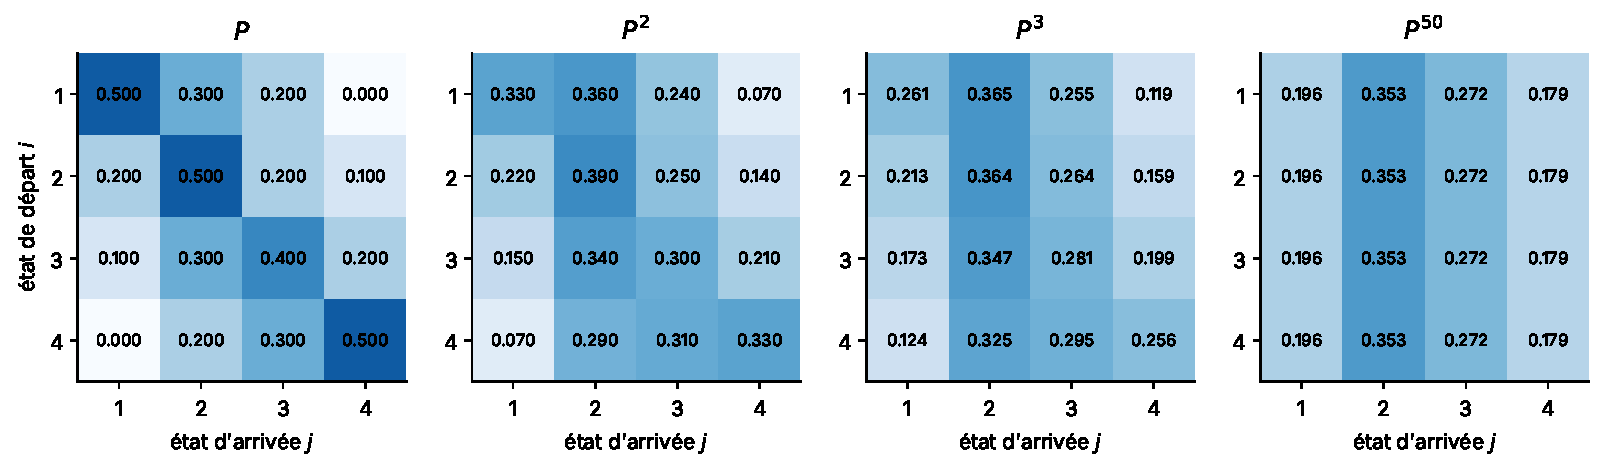
\includegraphics[width=\linewidth]{fig_markov_powers.pdf}
\caption{Puissances de la matrice de transition de l'exemple : $P$, $P^2$, $P^3$, $P^{50}$. Le coefficient $(i,j)$ de $P^n$ est la probabilité d'être en $j$ après $n$ pas en partant de $i$.}
\label{fig-markov}
\end{figure}

%=====================================================================
\section{Processus de décision markoviens}\label{sec-mdp}
%=====================================================================

\subsection{Définition}

Une chaîne de Markov décrit un système qui évolue seul. Un processus de décision markovien ajoute un décideur : la loi de l'état suivant dépend de l'état présent \emph{et} de l'action choisie.

\begin{definition}[MDP fini]\label{def-mdp}
Un processus de décision markovien fini est un quintuplet $\cM=(\cS,\cA,P,R,\gamma)$ où
\begin{itemize}
\item $\cS=\{s_1,\dots,s_n\}$ est un ensemble fini d'\emph{états} ;
\item $\cA=\{a_1,\dots,a_m\}$ est un ensemble fini d'\emph{actions} ;
\item $P$ est un \emph{noyau de transition} : pour tout $(s,a)$, $P(\cdot\mid s,a)$ est une loi de probabilité sur $\cS$, et $P(s'\mid s,a)$ est la probabilité d'arriver en $s'$ quand on joue $a$ en $s$ ;
\item $R:\cS\times\cA\times\cS\to\R$ est la \emph{fonction de récompense} ; on note $\Rmax=\max\abs{R(s,a,s')}$ ;
\item $\gamma\in[0,1)$ est le \emph{facteur d'actualisation}.
\end{itemize}
On note $r(s,a)=\sum_{s'}P(s'\mid s,a)R(s,a,s')$ la récompense moyenne immédiate.
\end{definition}

Pour chaque action $a$ fixée, la matrice $(P(s'\mid s,a))_{s,s'}$ est stochastique. Un MDP est donc une famille de $|\cA|$ chaînes de Markov entre lesquelles le décideur choisit à chaque pas.

\subsection{Politiques}

\begin{definition}[Politique]
Une \emph{politique stationnaire markovienne} (on dira simplement \emph{politique}) est une famille $\pi=(\pi(\cdot\mid s))_{s\in\cS}$ de lois sur $\cA$ : $\pi(a\mid s)\in[0,1]$ est la probabilité de choisir $a$ dans l'état $s$, et $\sum_a\pi(a\mid s)=1$. Elle est \emph{déterministe} s'il existe une fonction, encore notée $\pi:\cS\to\cA$, telle que $\pi(a\mid s)=\1\{a=\pi(s)\}$. On note $\Pi$ l'ensemble des politiques et $\Pi_D$ celui des politiques déterministes ; $\Pi_D$ est fini de cardinal $|\cA|^{|\cS|}$.
\end{definition}

Plus généralement, une politique pourrait dépendre de tout l'historique $(s_0,a_0,\dots,s_t)$ et du temps. On se restreint à $\Pi$ ; la \cref{rem-histoire} explique pourquoi ce n'est pas une perte de généralité.

\subsection{Loi des trajectoires et propriété de Markov}

Fixons une politique $\pi$ et un état initial $s$. Le mécanisme est : $S_0=s$ ; à chaque instant $t$, l'action $A_t$ est tirée selon $\pi(\cdot\mid S_t)$, puis l'état suivant $S_{t+1}$ selon $P(\cdot\mid S_t,A_t)$, et l'on reçoit $R_{t+1}=R(S_t,A_t,S_{t+1})$. Formellement, les lois fini-dimensionnelles sont
\begin{equation}\label{eq-loi-traj}
\begin{split}
&\P^\pi_s\big(S_0=s_0,A_0=a_0,\dots,S_t=s_t,A_t=a_t\big)\\
&\qquad=\1\{s_0=s\}\prod_{k=0}^{t}\pi(a_k\mid s_k)\prod_{k=0}^{t-1}P(s_{k+1}\mid s_k,a_k).
\end{split}
\end{equation}
Ces lois sont compatibles (sommer sur $a_t$ puis sur $s_t$ redonne la formule au rang précédent), et le théorème d'Ionescu-Tulcea garantit l'existence d'une unique probabilité $\P^\pi_s$ sur l'espace des trajectoires infinies qui les admet ; on l'admet. On note $\E^\pi_s$ l'espérance associée.

\begin{proposition}\label{prop-chaine-induite}
Sous $\P^\pi_s$, la suite des états $(S_t)$ est une chaîne de Markov de matrice
\[
P_\pi(s,s')=\sum_{a\in\cA}\pi(a\mid s)\,P(s'\mid s,a).
\]
\end{proposition}
\begin{proof}
En sommant \eqref{eq-loi-traj} sur $a_0,\dots,a_{t}$ (et en utilisant $\sum_{a_t}\pi(a_t\mid s_t)=1$), on obtient $\P^\pi_s(S_0=s_0,\dots,S_t=s_t)=\1\{s_0=s\}\prod_{k=0}^{t-1}P_\pi(s_k,s_{k+1})$. Le quotient de cette expression au rang $t+1$ par celle au rang $t$ vaut $P_\pi(s_t,s_{t+1})$ et ne dépend que de $s_t$ : c'est la propriété de Markov. La matrice $P_\pi$ est stochastique comme moyenne de matrices stochastiques.
\end{proof}

\paragraph{Pourquoi « markovien » ?} La loi de $(S_{t+1},R_{t+1})$ sachant tout le passé ne dépend que de $(S_t,A_t)$ : c'est l'hypothèse structurelle du modèle, visible dans \eqref{eq-loi-traj} où chaque facteur ne fait intervenir que l'état et l'action courants. C'est elle qui permettra la décomposition récursive de Bellman.

Nous utiliserons la conséquence suivante de \eqref{eq-loi-traj}.

\begin{lemme}[Redémarrage]\label{lem-redemarrage}
Pour tous $s,a,s'$ tels que $\pi(a\mid s)P(s'\mid s,a)>0$, la loi de la trajectoire décalée $(S_1,A_1,S_2,A_2,\dots)$ sous $\P^\pi_s(\,\cdot\mid A_0=a,S_1=s')$ est $\P^\pi_{s'}$.
\end{lemme}
\begin{proof}
D'après \eqref{eq-loi-traj}, pour toute suite $(s_1=s',a_1,\dots,s_{t},a_t)$,
\[
\begin{split}
&\P^\pi_s(A_0=a,S_1=s',A_1=a_1,\dots,S_t=s_t,A_t=a_t)\\
&\qquad=\pi(a\mid s)P(s'\mid s,a)\cdot\Big[\prod_{k=1}^{t}\pi(a_k\mid s_k)\prod_{k=1}^{t-1}P(s_{k+1}\mid s_k,a_k)\Big].
\end{split}
\]
En divisant par $\P^\pi_s(A_0=a,S_1=s')=\pi(a\mid s)P(s'\mid s,a)$, il reste le crochet, qui est exactement \eqref{eq-loi-traj} pour une trajectoire issue de $s'$. Les lois fini-dimensionnelles coïncident, donc les lois coïncident.
\end{proof}

\subsection{Retour actualisé et rôle de \texorpdfstring{$\gamma$}{gamma}}

\begin{definition}[Retour]
Le retour actualisé à partir de l'instant $t$ est
\[
G_t=R_{t+1}+\gamma R_{t+2}+\gamma^2R_{t+3}+\dots=\sum_{k=0}^{\infty}\gamma^kR_{t+k+1}.
\]
\end{definition}

\begin{proposition}[Bornitude du retour]\label{prop-borne-retour}
Si $\abs{R_t}\le\Rmax$ pour tout $t$ et $0\le\gamma<1$, la série définissant $G_t$ converge absolument pour toute trajectoire et
\[
\abs{G_t}\le\frac{\Rmax}{1-\gamma}.
\]
\end{proposition}
\begin{proof}
$\sum_k\abs{\gamma^kR_{t+k+1}}\le\Rmax\sum_k\gamma^k=\Rmax/(1-\gamma)<\infty$ par la \cref{prop-geom}. La série converge absolument, donc converge, et par l'inégalité triangulaire (passée à la limite sur les sommes partielles) $\abs{G_t}\le\sum_k\gamma^k\abs{R_{t+k+1}}\le\Rmax/(1-\gamma)$.
\end{proof}

\begin{proposition}[Relation récursive]\label{prop-recursion}
$G_t=R_{t+1}+\gamma G_{t+1}$.
\end{proposition}
\begin{proof}
$G_t=R_{t+1}+\sum_{k\ge1}\gamma^kR_{t+k+1}=R_{t+1}+\gamma\sum_{j\ge0}\gamma^jR_{t+1+j+1}=R_{t+1}+\gamma G_{t+1}$, le réindexage $j=k-1$ étant licite pour une série absolument convergente.
\end{proof}

\paragraph{Pourquoi impose-t-on $\gamma<1$ ?} Trois raisons, de natures différentes, convergent.
\begin{enumerate}
\item \emph{Analytique.} Avec $\gamma=1$, la somme des récompenses peut diverger (récompenses $-1$ à chaque pas d'une politique qui tourne en rond indéfiniment), et $V^\pi$ n'est plus défini. Avec $\gamma<1$ et des récompenses bornées, tout est fini (\cref{prop-borne-retour}).
\item \emph{Probabiliste.} Soit $\tau$ une variable géométrique indépendante de la trajectoire, $\P(\tau>k)=\gamma^k$ (à chaque pas, le processus « s'arrête » avec probabilité $1-\gamma$). Alors, pour des récompenses bornées, $\E\big[\sum_{k=0}^{\tau-1}R_{k+1}\big]=\E\big[\sum_{k\ge0}\1\{\tau>k\}R_{k+1}\big]=\E\big[\sum_k\gamma^kR_{k+1}\big]$ (indépendance et Fubini, justifié par la domination $\sum_k\gamma^k\Rmax$). Actualiser revient donc à maximiser la somme non actualisée sur un horizon aléatoire de durée moyenne $1/(1-\gamma)$ ; par exemple $1/(1-\gamma)=10$ pour $\gamma=0.9$ et $100$ pour $\gamma=0.99$.
\item \emph{Algorithmique.} On verra que $\gamma$ est exactement le rapport de contraction de l'opérateur de Bellman (\cref{thm-contraction}). C'est $\gamma<1$ qui rend applicable le théorème de Banach.
\end{enumerate}
Plus $\gamma$ est proche de $0$, plus l'agent est « myope » ; plus il est proche de $1$, plus il valorise le long terme, au prix d'une convergence plus lente.

%=====================================================================
\section{Fonctions de valeur}\label{sec-valeurs}
%=====================================================================

\begin{definition}
Pour une politique $\pi$, la \emph{fonction de valeur} et la \emph{fonction d'action-valeur} (fonction $Q$) sont
\[
V^\pi(s)=\E^\pi_s[G_0],\qquad
Q^\pi(s,a)=\E^\pi_s[G_0\mid A_0=a]\quad(\text{si }\pi(a\mid s)>0).
\]
\end{definition}

Comme $G_0$ est bornée, ces espérances existent. Par stationnarité, $V^\pi(s)$ est aussi l'espérance de $G_t$ sachant $S_t=s$ pour n'importe quel $t$, ce qui justifie la notation du cahier des charges $V^\pi(s)=\E_\pi[G_t\mid S_t=s]$.

\paragraph{Interprétation.} $V^\pi(s)$ est la récompense totale actualisée moyenne obtenue en partant de $s$ et en suivant $\pi$. $Q^\pi(s,a)$ est la même quantité quand on impose la première action $a$ et qu'on suit $\pi$ ensuite : elle mesure la \emph{qualité} de l'action $a$ dans l'état $s$. La différence est essentielle pour la suite : connaître $V^\pi$ ne suffit pas pour choisir une action sans connaître le modèle $P$, alors que connaître $Q$ permet de choisir $\argmax_a Q(s,a)$ directement. C'est pour cela que le Q-Learning apprend $Q$ et non $V$.

Pour que $Q^\pi(s,a)$ soit défini même lorsque $\pi(a\mid s)=0$, on pose directement
\begin{equation}\label{eq-Q-from-V}
\begin{split}
Q^\pi(s,a)&=\sum_{s'}P(s'\mid s,a)\big[R(s,a,s')+\gamma V^\pi(s')\big]\\
&=r(s,a)+\gamma\sum_{s'}P(s'\mid s,a)V^\pi(s'),
\end{split}
\end{equation}
la \cref{prop-VQ} montrant que cela coïncide avec l'espérance conditionnelle lorsque $\pi(a\mid s)>0$.

\begin{proposition}\label{prop-VQ}
Pour toute politique $\pi$ et tout $s$ :
\begin{enumerate}[label=(\alph*)]
\item si $\pi(a\mid s)>0$, $\E^\pi_s[G_0\mid A_0=a]=\sum_{s'}P(s'\mid s,a)\big[R(s,a,s')+\gamma V^\pi(s')\big]$ ;
\item $V^\pi(s)=\sum_a\pi(a\mid s)\,Q^\pi(s,a)$.
\end{enumerate}
\end{proposition}
\begin{proof}
(a) Par la \cref{prop-recursion}, $G_0=R_1+\gamma G_1$ avec $R_1=R(s,a,S_1)$ sur $\{A_0=a\}$. On conditionne par la valeur de $S_1$ (\cref{lem-totale}) :
\[
\E^\pi_s[G_0\mid A_0=a]=\sum_{s'}P(s'\mid s,a)\Big(R(s,a,s')+\gamma\,\E^\pi_s[G_1\mid A_0=a,S_1=s']\Big),
\]
car $\P^\pi_s(S_1=s'\mid A_0=a)=P(s'\mid s,a)$ d'après \eqref{eq-loi-traj}. Or $G_1=\sum_k\gamma^kR(S_{k+1},A_{k+1},S_{k+2})$ est la même fonction de la trajectoire décalée que $G_0$ de la trajectoire initiale. D'après le \cref{lem-redemarrage}, la trajectoire décalée a pour loi $\P^\pi_{s'}$, donc $\E^\pi_s[G_1\mid A_0=a,S_1=s']=\E^\pi_{s'}[G_0]=V^\pi(s')$. (Si $P(s'\mid s,a)=0$, le terme est nul et n'intervient pas.)

(b) On conditionne $G_0$ par la valeur de $A_0$, de loi $\pi(\cdot\mid s)$ (\cref{lem-totale}), et on utilise (a) pour les $a$ tels que $\pi(a\mid s)>0$ ; les autres ont un poids nul.
\end{proof}

%=====================================================================
\section{Équations de Bellman}\label{sec-bellman}
%=====================================================================

\subsection{Équation de Bellman pour une politique fixée}

En combinant les deux points de la \cref{prop-VQ}, on obtient le résultat suivant.

\begin{theoreme}[Équations de Bellman d'évaluation]\label{thm-bellman-pi}
Pour toute politique $\pi$ et tous $s\in\cS$, $a\in\cA$,
\begin{align}
V^\pi(s)&=\sum_a\pi(a\mid s)\sum_{s'}P(s'\mid s,a)\big[R(s,a,s')+\gamma V^\pi(s')\big]
=\E^\pi_s\big[R_1+\gamma V^\pi(S_1)\big],\label{eq-bellman-V}\\
Q^\pi(s,a)&=\sum_{s'}P(s'\mid s,a)\Big[R(s,a,s')+\gamma\sum_{a'}\pi(a'\mid s')Q^\pi(s',a')\Big].\label{eq-bellman-Q}
\end{align}
\end{theoreme}
\begin{proof}
\eqref{eq-bellman-V} : injecter \eqref{eq-Q-from-V} dans la \cref{prop-VQ}(b). \eqref{eq-bellman-Q} : injecter la \cref{prop-VQ}(b), appliquée en $s'$, dans \eqref{eq-Q-from-V}.
\end{proof}

L'idée est simple : la valeur d'un état est la récompense immédiate moyenne plus $\gamma$ fois la valeur moyenne de l'état suivant. Le problème sur un horizon infini se ramène à un problème à un pas, grâce à la propriété de Markov.

\paragraph{Forme matricielle et unicité.} Notons $r_\pi(s)=\sum_a\pi(a\mid s)r(s,a)$. L'équation \eqref{eq-bellman-V} s'écrit
\[
V^\pi=r_\pi+\gamma P_\pi V^\pi\iff(I-\gamma P_\pi)V^\pi=r_\pi.
\]

\begin{proposition}\label{prop-neumann}
$I-\gamma P_\pi$ est inversible, et
\[
V^\pi=(I-\gamma P_\pi)^{-1}r_\pi=\sum_{k=0}^{\infty}\gamma^kP_\pi^k\,r_\pi.
\]
\end{proposition}
\begin{proof}
Pour la norme d'opérateur subordonnée à $\ninf\cdot$, $\norm{P_\pi}=\max_s\sum_{s'}P_\pi(s,s')=1$ car $P_\pi$ est stochastique (\cref{lem-moyenne}), donc $\norm{\gamma P_\pi}=\gamma<1$. La série de Neumann $\sum_k(\gamma P_\pi)^k$ converge alors normalement (\cref{prop-geom}), et un calcul télescopique montre que sa somme $N$ vérifie $(I-\gamma P_\pi)N=N(I-\gamma P_\pi)=I$.
\end{proof}

La formule a une lecture probabiliste immédiate : par Chapman-Kolmogorov (\cref{thm-ck,prop-chaine-induite}), $(P_\pi^kr_\pi)(s)=\E^\pi_s[r_\pi(S_k)]=\E^\pi_s[R_{k+1}]$ est la récompense moyenne reçue au pas $k+1$. Ainsi $V^\pi(s)=\sum_k\gamma^k\E^\pi_s[R_{k+1}]$ : la série des espérances. Le code utilise cette proposition pour évaluer exactement une politique (\texttt{evaluate\_policy\_exact}), en résolvant un système linéaire $14\times14$.

\subsection{Équation d'optimalité de Bellman}

\begin{definition}[Valeurs optimales]
\[
V^*(s)=\sup_{\pi\in\Pi}V^\pi(s),\qquad Q^*(s,a)=\sup_{\pi\in\Pi}Q^\pi(s,a).
\]
Une politique $\pi^*$ est \emph{optimale} si $V^{\pi^*}(s)=V^*(s)$ pour tout $s$.
\end{definition}

Ces bornes supérieures sont finies puisque $\abs{V^\pi}\le\Rmax/(1-\gamma)$. A priori, rien ne dit qu'une même politique réalise le $\sup$ simultanément en tous les états. L'heuristique de Bellman (principe d'optimalité) suggère pourtant que, si l'on agit optimalement à partir du pas suivant, il suffit de choisir au pas présent l'action qui maximise « récompense immédiate $+\ \gamma\times$ valeur optimale de l'état suivant ». Cela conduit à l'\emph{équation d'optimalité}
\begin{equation}\label{eq-bellman-opt}
\begin{split}
Q^*(s,a)&=\sum_{s'}P(s'\mid s,a)\Big[R(s,a,s')+\gamma\max_{a'}Q^*(s',a')\Big]\\
&=\E\Big[R_{t+1}+\gamma\max_{a'}Q^*(S_{t+1},a')\;\Big|\;S_t=s,A_t=a\Big].
\end{split}
\end{equation}
Cette équation est non linéaire à cause du $\max$ : on ne peut plus la résoudre par inversion de matrice. La section suivante démontre rigoureusement qu'elle a une unique solution, que cette solution est bien $Q^*$, et qu'une politique gloutonne pour $Q^*$ est optimale. L'outil sera le théorème de Banach.

%=====================================================================
\section{Opérateur de Bellman et contraction}\label{sec-operateur}
%=====================================================================

\subsection{Définitions}

On travaille dans l'espace $\mathcal{Q}=\R^{\cS\times\cA}$ des fonctions $Q:\cS\times\cA\to\R$, muni de la norme infinie. C'est un espace vectoriel de dimension finie $d=|\cS||\cA|$, complet d'après la \cref{prop-complet}.

\begin{definition}[Opérateurs de Bellman]
Pour $Q\in\mathcal{Q}$ et une politique $\pi$, on définit $TQ,\,T^\pi Q\in\mathcal Q$ par
\begin{align*}
(TQ)(s,a)&=\sum_{s'}P(s'\mid s,a)\Big[R(s,a,s')+\gamma\max_{a'}Q(s',a')\Big]\\
&=r(s,a)+\gamma\sum_{s'}P(s'\mid s,a)\max_{a'}Q(s',a'),\\
(T^\pi Q)(s,a)&=r(s,a)+\gamma\sum_{s'}P(s'\mid s,a)\sum_{a'}\pi(a'\mid s')\,Q(s',a').
\end{align*}
\end{definition}

Avec ces notations, l'équation \eqref{eq-bellman-Q} s'écrit $T^\pi Q^\pi=Q^\pi$ et l'équation d'optimalité \eqref{eq-bellman-opt} s'écrit
\[
\boxed{TQ^*=Q^*}
\]
autrement dit : \emph{$Q^*$ est un point fixe de l'opérateur de Bellman}. Le problème de contrôle optimal devient un problème de point fixe.

\subsection{Propriétés élémentaires}

On note $Q_1\le Q_2$ si $Q_1(s,a)\le Q_2(s,a)$ pour tout $(s,a)$, et $\1$ la fonction constante égale à $1$.

\begin{lemme}\label{lem-proprietes}
Pour tous $Q,Q_1,Q_2\in\mathcal Q$, toute politique $\pi$ et toute constante $c\in\R$ :
\begin{enumerate}[label=(\roman*)]
\item \emph{monotonie} : $Q_1\le Q_2\Rightarrow TQ_1\le TQ_2$ et $T^\pi Q_1\le T^\pi Q_2$ ;
\item \emph{translation} : $T(Q+c\1)=TQ+\gamma c\1$ et $T^\pi(Q+c\1)=T^\pi Q+\gamma c\1$ ;
\item \emph{domination} : $T^\pi Q\le TQ$, avec égalité si $\pi$ est gloutonne pour $Q$, c'est-à-dire si $\pi(\cdot\mid s)$ ne charge que des actions de $\argmax_{a'}Q(s,a')$.
\end{enumerate}
\end{lemme}
\begin{proof}
(i) Si $Q_1\le Q_2$, alors $\max_{a'}Q_1(s',a')\le\max_{a'}Q_2(s',a')$ pour tout $s'$, et une combinaison à coefficients positifs préserve l'inégalité. Même raisonnement pour $T^\pi$. (ii) $\max_{a'}(Q(s',a')+c)=\max_{a'}Q(s',a')+c$ et $\sum_{s'}P(s'\mid s,a)\,c=c$. (iii) Une moyenne est inférieure au maximum : $\sum_{a'}\pi(a'\mid s')Q(s',a')\le\max_{a'}Q(s',a')$, avec égalité exactement quand $\pi(\cdot\mid s')$ est portée par les maximiseurs.
\end{proof}

\subsection{Le théorème de contraction}

\begin{theoreme}[Contraction de l'opérateur de Bellman]\label{thm-contraction}
Pour tous $Q_1,Q_2\in\mathcal Q$,
\[
\ninf{TQ_1-TQ_2}\le\gamma\,\ninf{Q_1-Q_2}\qquad\text{et}\qquad\ninf{T^\pi Q_1-T^\pi Q_2}\le\gamma\,\ninf{Q_1-Q_2}.
\]
Comme $0\le\gamma<1$, $T$ et $T^\pi$ sont des contractions de $(\mathcal Q,\ninf\cdot)$ de rapport $\gamma$.
\end{theoreme}
\begin{proof}
Fixons $(s,a)$. Les récompenses $r(s,a)$ sont identiques dans $TQ_1$ et $TQ_2$ et disparaissent dans la différence :
\[
(TQ_1)(s,a)-(TQ_2)(s,a)=\gamma\sum_{s'}P(s'\mid s,a)\Big[\max_{a'}Q_1(s',a')-\max_{a'}Q_2(s',a')\Big].
\]
On prend la valeur absolue et on enchaîne trois inégalités.
\begin{align*}
\abs{(TQ_1)(s,a)-(TQ_2)(s,a)}
&\le\gamma\sum_{s'}P(s'\mid s,a)\,\Big|\max_{a'}Q_1(s',a')-\max_{a'}Q_2(s',a')\Big| &&\text{(a)}\\
&\le\gamma\sum_{s'}P(s'\mid s,a)\,\max_{a'}\abs{Q_1(s',a')-Q_2(s',a')} &&\text{(b)}\\
&\le\gamma\sum_{s'}P(s'\mid s,a)\,\ninf{Q_1-Q_2} &&\text{(c)}\\
&=\gamma\,\ninf{Q_1-Q_2} &&\text{(d)}
\end{align*}
Les justifications sont : (a) inégalité triangulaire et positivité des $P(s'\mid s,a)$ ; (b) \cref{lem-max} appliqué à $f=Q_1(s',\cdot)$ et $g=Q_2(s',\cdot)$ ; (c) définition de $\ninf\cdot$, puisque $\abs{Q_1(s',a')-Q_2(s',a')}\le\ninf{Q_1-Q_2}$ pour tout $(s',a')$ ; (d) $\sum_{s'}P(s'\mid s,a)=1$. Le membre de droite ne dépend pas de $(s,a)$ ; en prenant le maximum sur $(s,a)$ à gauche, on obtient l'inégalité annoncée. Pour $T^\pi$, on remplace la deuxième ligne par $\abs{\sum_{a'}\pi(a'\mid s')(Q_1-Q_2)(s',a')}\le\ninf{Q_1-Q_2}$ (\cref{lem-moyenne}).
\end{proof}

\paragraph{D'où vient le facteur $\gamma$ ?} La preuve montre que chaque ingrédient de $T$ joue un rôle précis : la récompense s'annule dans la différence, le $\max$ ne dilate pas les écarts (\cref{lem-max}), l'espérance sur $s'$ non plus (\cref{lem-moyenne}). La seule opération qui modifie l'écart est la multiplication par $\gamma$. Le rapport de contraction est donc exactement $\gamma$, sans dépendance au nombre d'états ni à la structure de $P$.

\begin{remarque}[La constante $\gamma$ est optimale]
Avec $Q_2=Q_1+c\1$, le \cref{lem-proprietes}(ii) donne $\ninf{TQ_2-TQ_1}=\gamma\abs c=\gamma\ninf{Q_2-Q_1}$ : on ne peut pas remplacer $\gamma$ par une constante plus petite. Numériquement (\cref{fig-vi}, à droite), sur $20\,000$ couples aléatoires par valeur de $\gamma$, le rapport $\ninf{TQ_1-TQ_2}/\ninf{Q_1-Q_2}$ n'a jamais dépassé $\gamma$ (maximum observé $\ContrMaxNine$ pour $\gamma=0.9$) et vaut $\ContrEqNine$ dans le cas d'égalité ; sa moyenne ($\ContrMeanNine$) est nettement plus faible, car pour des $Q$ quelconques le \cref{lem-max} est en général strict.
\end{remarque}

\subsection{Existence, unicité et caractérisation de \texorpdfstring{$Q^*$}{Q*}}

\begin{theoreme}[Point fixe de Bellman et optimalité]\label{thm-optimalite}
\begin{enumerate}[label=(\alph*)]
\item Pour toute politique $\pi$, $Q^\pi$ est l'unique point fixe de $T^\pi$.
\item $T$ possède un unique point fixe, noté $\bar Q$.
\item Pour toute politique $\pi\in\Pi$, $Q^\pi\le\bar Q$.
\item Toute politique déterministe gloutonne pour $\bar Q$, $\bar\pi(s)\in\argmax_a\bar Q(s,a)$, vérifie $Q^{\bar\pi}=\bar Q$.
\end{enumerate}
Par conséquent $Q^*=\bar Q$ : la fonction $Q^*$ définie comme borne supérieure est l'unique solution de l'équation d'optimalité $TQ=Q$, cette borne supérieure est atteinte simultanément en tous les $(s,a)$ par la politique déterministe $\bar\pi$, et l'on a $V^*(s)=\max_aQ^*(s,a)$ ; $\bar\pi$ est optimale.
\end{theoreme}
\begin{proof}
(a) Par le \cref{thm-bellman-pi}, $T^\pi Q^\pi=Q^\pi$. Par le \cref{thm-contraction}, $T^\pi$ est une contraction de l'espace complet $\mathcal Q$ ; par le \cref{thm-banach}, son point fixe est unique.

(b) Même argument pour $T$ (\cref{thm-contraction,thm-banach}).

(c) Par (a) et le \cref{lem-proprietes}(iii), $Q^\pi=T^\pi Q^\pi\le TQ^\pi$. En appliquant $T$, qui est monotone (\cref{lem-proprietes}(i)), on obtient $TQ^\pi\le T^2Q^\pi$, puis par récurrence $Q^\pi\le TQ^\pi\le T^2Q^\pi\le\dots\le T^kQ^\pi$ pour tout $k$. D'après le \cref{thm-banach}(ii), $T^kQ^\pi\to\bar Q$ ; les inégalités larges passent à la limite coordonnée par coordonnée, d'où $Q^\pi\le\bar Q$.

(d) Si $\bar\pi$ est gloutonne pour $\bar Q$, le \cref{lem-proprietes}(iii) donne $T^{\bar\pi}\bar Q=T\bar Q=\bar Q$. Donc $\bar Q$ est un point fixe de $T^{\bar\pi}$, et par l'unicité (a), $\bar Q=Q^{\bar\pi}$.

\emph{Conclusion.} (c) donne $Q^*=\sup_\pi Q^\pi\le\bar Q$ et (d) donne $\bar Q=Q^{\bar\pi}\le Q^*$, donc $Q^*=\bar Q$ et le $\sup$ est atteint par $\bar\pi$. Pour les valeurs d'état, la \cref{prop-VQ}(b) et (c) donnent $V^\pi(s)=\sum_a\pi(a\mid s)Q^\pi(s,a)\le\max_a\bar Q(s,a)$, et pour $\bar\pi$ déterministe gloutonne $V^{\bar\pi}(s)=Q^{\bar\pi}(s,\bar\pi(s))=\bar Q(s,\bar\pi(s))=\max_a\bar Q(s,a)$. D'où $V^*(s)=\max_aQ^*(s,a)=V^{\bar\pi}(s)$.
\end{proof}

La chaîne logique centrale du projet est désormais établie :
\[
\boxed{\begin{array}{c}
T\text{ contraction de rapport }\gamma\;\Longrightarrow\;\text{point fixe unique (Banach)}\\[2pt]
\Longrightarrow\;\text{ce point fixe est }Q^*\;\Longrightarrow\;\pi^*(s)\in\argmax_aQ^*(s,a)\text{ est optimale.}
\end{array}}
\]

\begin{remarque}[Politiques dépendant de l'historique]\label{rem-histoire}
On s'est restreint aux politiques stationnaires markoviennes. Le résultat reste vrai si l'on autorise des politiques qui dépendent de tout l'historique et du temps, même randomisées : aucune ne fait mieux que $\bar\pi$ (Puterman, 1994, théorème 6.2.10). La preuve, plus technique, n'est pas reproduite ici.
\end{remarque}

\begin{remarque}[Vérifications numériques]
Sur notre GridWorld (\cref{sec-experiences}), on a vérifié que l'évaluation exacte de la politique gloutonne pour $Q^*$ redonne $Q^*$ à $\NumGreedyMatch$ près (point (d)), et que, pour $\NumRandomPolicies$ politiques tirées au hasard (moitié déterministes, moitié stochastiques), $\max_{s,a}(Q^\pi-Q^*)(s,a)=\NumMaxQpiMinusQstar$, c'est-à-dire zéro aux erreurs d'arrondi près (point (c)). La meilleure de ces politiques aléatoires n'atteint que $V^\pi(S)=\NumBestRandom$ contre $V^*(S)=\VstarS$.
\end{remarque}

\subsection{Qualité d'une politique gloutonne approchée}

En pratique on ne dispose que d'une approximation $Q\approx Q^*$. Le résultat suivant, dans l'esprit de Singh et Yee (1994), contrôle la perte.

\begin{proposition}\label{prop-perte}
Soit $Q\in\mathcal Q$ avec $\ninf{Q-Q^*}\le\varepsilon$ et $\pi$ une politique déterministe gloutonne pour $Q$. Alors
\[
0\le V^*(s)-V^{\pi}(s)\le\frac{2\varepsilon}{1-\gamma}\qquad\text{pour tout }s.
\]
De plus, si $\varepsilon<\Delta/2$, où $\Delta=\min_s\big(\max_aQ^*(s,a)-\max_{a\notin\mathcal A^*(s)}Q^*(s,a)\big)>0$ est le plus petit écart d'action ($\mathcal A^*(s)$ désignant l'ensemble des actions optimales en $s$, le minimum portant sur les états où $\mathcal A^*(s)\neq\cA$), alors $\pi$ est optimale.
\end{proposition}
\begin{proof}
Soit $s$, $a=\pi(s)$ et $a^*\in\mathcal A^*(s)$. Comme $Q(s,a)\ge Q(s,a^*)$,
\[
Q^*(s,a^*)-Q^*(s,a)\le\big(Q(s,a^*)+\varepsilon\big)-\big(Q(s,a)-\varepsilon\big)\le2\varepsilon.
\]
En utilisant \eqref{eq-Q-from-V} pour $Q^*=Q^{\bar\pi}$ et pour $Q^\pi$,
\[
V^*(s)-V^\pi(s)=Q^*(s,a^*)-Q^\pi(s,a)=\big[Q^*(s,a^*)-Q^*(s,a)\big]+\gamma\sum_{s'}P(s'\mid s,a)\big[V^*(s')-V^\pi(s')\big].
\]
Le premier crochet est au plus $2\varepsilon$, le second terme au plus $\gamma\ninf{V^*-V^\pi}$. En passant au maximum sur $s$, $\ninf{V^*-V^\pi}\le2\varepsilon+\gamma\ninf{V^*-V^\pi}$, d'où la borne. La positivité vient de la définition de $V^*$. Pour le second point, si $a\notin\mathcal A^*(s)$ on aurait $Q^*(s,a^*)-Q^*(s,a)\ge\Delta>2\varepsilon$, ce qui contredit l'inégalité ci-dessus ; donc $\pi(s)\in\mathcal A^*(s)$ pour tout $s$, et $\pi$ est gloutonne pour $Q^*$, donc optimale par le \cref{thm-optimalite}(d).
\end{proof}

Sur notre GridWorld, l'écart d'action vaut $\Delta=\ActionGap$. Il suffit donc de connaître $Q^*$ à moins de $\ActionGapHalf$ près, uniformément, pour en déduire une politique optimale. Ce seuil servira à lire les courbes d'erreur de la \cref{sec-experiences}.

%=====================================================================
\section{Value Iteration}\label{sec-vi}
%=====================================================================

\subsection{Algorithme}

Value Iteration consiste simplement à itérer l'opérateur de Bellman à partir d'un $Q_0$ quelconque (on prend $Q_0=0$) :
\[
Q_{k+1}(s,a)=(TQ_k)(s,a)=\sum_{s'}P(s'\mid s,a)\Big[R(s,a,s')+\gamma\max_{a'}Q_k(s',a')\Big].
\]

\begin{algorithm}[ht]
\caption{Value Iteration (fonction \texttt{value\_iteration})}
\KwIn{$P$, $R$, $\gamma\in[0,1)$, tolérance $\eta>0$}
$Q_0\leftarrow0$, $k\leftarrow0$\;
\Repeat{$\ninf{Q_{k}-Q_{k-1}}<\eta$}{
  \For{$(s,a)\in\cS\times\cA$}{
    $Q_{k+1}(s,a)\leftarrow\sum_{s'}P(s'\mid s,a)\big[R(s,a,s')+\gamma\max_{a'}Q_k(s',a')\big]$\;
  }
  $k\leftarrow k+1$\;
}
\KwOut{$Q_k\approx Q^*$ et la politique gloutonne $\pi(s)=\argmax_aQ_k(s,a)$}
\end{algorithm}

\subsection{Démonstration de convergence}

\begin{theoreme}[Convergence de Value Iteration]\label{thm-vi}
Pour tout $Q_0$, la suite $Q_{k+1}=TQ_k$ converge vers $Q^*$ et, pour tout $k$,
\[
\ninf{Q_k-Q^*}\le\gamma^k\ninf{Q_0-Q^*},\qquad
\ninf{Q_{k+1}-Q^*}\le\frac{\gamma}{1-\gamma}\ninf{Q_{k+1}-Q_k}.
\]
En particulier, si l'algorithme s'arrête dès que $\ninf{Q_{k+1}-Q_k}<\eta$, l'erreur finale est inférieure à $\gamma\eta/(1-\gamma)$. Enfin, la politique gloutonne pour $Q_k$ est optimale dès que $\gamma^k\ninf{Q_0-Q^*}<\Delta/2$, donc après un nombre fini d'itérations.
\end{theoreme}
\begin{proof}
C'est le \cref{thm-banach} appliqué à $T$ (\cref{thm-contraction}), sur l'espace complet $\mathcal Q$ (\cref{prop-complet}), dont le point fixe est $Q^*$ (\cref{thm-optimalite}). La dernière affirmation découle de la \cref{prop-perte}.
\end{proof}

\paragraph{Ce que le théorème ne dit pas : la vitesse réelle.} La borne $\gamma^k$ est un pire cas. Sur notre exemple, le rapport $\ninf{Q_{k+1}-Q^*}/\ninf{Q_k-Q^*}$ se stabilise vers $\VIRatioLast$, bien en dessous de $\gamma=0.9$ (\cref{fig-vi}). L'explication est la suivante. Une fois que les actions gloutonnes de $Q_k$ coïncident avec celles de $Q^*$ (ce qui arrive en un nombre fini d'itérations), on a $\max_{a'}Q_k(s',a')-\max_{a'}Q^*(s',a')=(Q_k-Q^*)(s',\pi^*(s'))$, et l'erreur évolue \emph{linéairement} : $e_{k+1}=\gamma PE_{\pi^*}e_k$, où $E_{\pi^*}$ sélectionne l'action optimale. L'erreur sur l'état absorbant $G$ est nulle, et le taux asymptotique est $\gamma\,\rho$, où $\rho$ est le rayon spectral de la matrice $P_{\pi^*}$ restreinte aux états non terminaux. Ici $\rho=\SpectralRho$ et $\gamma\rho=\AsymptoticRate$, ce qui correspond exactement au rapport observé. Intuitivement, la masse de probabilité « fuit » vers l'état absorbant, ce qui accélère la contraction au-delà de ce que garantit $\gamma$ seul. (Cet argument suppose une politique optimale unique en chaque état ; en l'état $S$, deux actions sont optimales par symétrie, ce qui ne change pas la conclusion observée.)

%=====================================================================
\section{Q-Learning}\label{sec-qlearning}
%=====================================================================

\subsection{Pourquoi un autre algorithme ?}

Value Iteration exige de connaître $P(s'\mid s,a)$ et $R(s,a,s')$ pour calculer l'espérance qui définit $T$. Dans beaucoup de problèmes, ce modèle est inconnu : l'agent ne peut qu'agir et observer des transitions $(s_t,a_t,r_t,s_{t+1})$. L'idée du Q-Learning est de remplacer l'espérance inconnue par l'échantillon observé, et de compenser le bruit ainsi introduit par une moyenne progressive.

\subsection{Algorithme}

\begin{algorithm}[ht]
\caption{Q-Learning tabulaire (fonction \texttt{q\_learning})}
\KwIn{$\gamma$, suite de pas $\alpha$, paramètre d'exploration $\varepsilon$, nombre d'épisodes}
$Q(s,a)\leftarrow0$ pour tout $(s,a)$ ; $N(s,a)\leftarrow0$\;
\For{chaque épisode}{
  $s\leftarrow$ état initial\;
  \Repeat{$s$ terminal ou nombre maximal de pas atteint}{
    choisir $a$ selon la politique $\varepsilon$-gloutonne pour $Q$ en $s$\;
    exécuter $a$ ; observer $r$ et $s'$\;
    $N(s,a)\leftarrow N(s,a)+1$ ; $\alpha\leftarrow\alpha(N(s,a))$\;
    $\delta\leftarrow r+\gamma\max_{a'}Q(s',a')-Q(s,a)$ \tcp*{avec $\max_{a'}Q(s',a')=0$ si $s'$ terminal}
    $Q(s,a)\leftarrow Q(s,a)+\alpha\,\delta$\;
    $s\leftarrow s'$\;
  }
}
\end{algorithm}

L'algorithme n'utilise jamais $P$ ni $R$ : seulement la fonction \texttt{step} de l'environnement. Dans le code, le modèle n'est utilisé que pour \emph{mesurer} l'erreur $\ninf{Q_t-Q^*}$ et la valeur des politiques apprises, jamais pour apprendre (un test unitaire vérifie que l'apprentissage fonctionne avec un modèle rendu illisible).

\subsection{L'erreur temporelle}

On note
\[
\delta_t=r_t+\gamma\max_aQ_t(s_{t+1},a)-Q_t(s_t,a_t),\qquad Q_{t+1}(s_t,a_t)=Q_t(s_t,a_t)+\alpha_t\delta_t,
\]
les autres coordonnées restant inchangées. La quantité $y_t=r_t+\gamma\max_aQ_t(s_{t+1},a)$ est la \emph{cible} : c'est une estimation, construite à partir d'une seule transition, de $(TQ_t)(s_t,a_t)$. L'erreur temporelle (\emph{TD error}) $\delta_t=y_t-Q_t(s_t,a_t)$ mesure l'écart entre ce que $Q_t$ prédit pour $(s_t,a_t)$ et ce que l'équation de Bellman, évaluée sur la transition observée, suggère. Si $Q_t=Q^*$, l'équation d'optimalité dit que cette cible vaut $Q^*(s_t,a_t)$ \emph{en moyenne} ; $\delta_t$ n'est alors qu'un bruit centré. La proposition suivante rend ceci précis.

Soit $\cF_t$ la tribu engendrée par toute l'histoire jusqu'au choix de $a_t$ inclus : $(s_0,a_0,r_0,\dots,s_t,a_t)$. La fonction $Q_t$ est $\cF_t$-mesurable (elle est calculée à partir des transitions passées), et, par la propriété de Markov du MDP, la loi conditionnelle de $s_{t+1}$ sachant $\cF_t$ est $P(\cdot\mid s_t,a_t)$, avec $r_t=R(s_t,a_t,s_{t+1})$.

\begin{proposition}[Espérance de l'erreur TD]\label{prop-td}
\[
\E\big[y_t\mid\cF_t\big]=(TQ_t)(s_t,a_t)\qquad\text{et donc}\qquad\E\big[\delta_t\mid\cF_t\big]=(TQ_t-Q_t)(s_t,a_t).
\]
\end{proposition}
\begin{proof}
Conditionnellement à $\cF_t$, les quantités $s_t,a_t,Q_t$ sont fixées et seul $s_{t+1}$ est aléatoire, de loi $P(\cdot\mid s_t,a_t)$. Donc
\[
\E[y_t\mid\cF_t]=\sum_{s'}P(s'\mid s_t,a_t)\Big[R(s_t,a_t,s')+\gamma\max_aQ_t(s',a)\Big]=(TQ_t)(s_t,a_t),
\]
et $Q_t(s_t,a_t)$ étant $\cF_t$-mesurable, il sort de l'espérance conditionnelle.
\end{proof}

On peut donc réécrire la mise à jour sous la forme d'une \emph{itération de point fixe bruitée et relaxée} :
\begin{equation}\label{eq-sa-form}
Q_{t+1}(s_t,a_t)=(1-\alpha_t)\,Q_t(s_t,a_t)+\alpha_t\Big[(TQ_t)(s_t,a_t)+w_t\Big],\qquad w_t=y_t-(TQ_t)(s_t,a_t),
\end{equation}
où le bruit $w_t$ vérifie $\E[w_t\mid\cF_t]=0$. De plus, $\abs{y_t}\le\Rmax+\gamma\ninf{Q_t}$ et $\abs{(TQ_t)(s_t,a_t)}\le\Rmax+\gamma\ninf{Q_t}$, donc
\begin{equation}\label{eq-var-bound}
\E[w_t^2\mid\cF_t]\le4\big(\Rmax+\gamma\ninf{Q_t}\big)^2\le C\big(1+\ninf{Q_t}^2\big).
\end{equation}

La forme \eqref{eq-sa-form} éclaire la relation entre les deux algorithmes.
\begin{itemize}
\item Si l'on mettait à jour \emph{toutes} les paires à chaque pas, avec $\alpha_t=1$ et sans bruit ($w_t=0$), on retrouverait exactement Value Iteration $Q_{t+1}=TQ_t$.
\item Q-Learning est \emph{asynchrone} (une seule coordonnée mise à jour par pas, celle que l'agent vient de visiter), \emph{bruité} (on utilise un échantillon au lieu de l'espérance) et \emph{relaxé} (on ne fait qu'un pas de taille $\alpha_t$ vers la cible).
\item La correction se fait dans la direction de $\delta_t$ : si la cible est au-dessus de l'estimation, on augmente $Q(s_t,a_t)$, sinon on la diminue. Le pas $\alpha_t$ règle le compromis entre réactivité (grand $\alpha$) et stabilité face au bruit (petit $\alpha$).
\end{itemize}

\subsection{Taux d'apprentissage : les conditions de Robbins-Monro}\label{sec-rm}

Pour comprendre le rôle de $\alpha_t$ sans la complexité du Q-Learning, considérons le problème le plus simple d'approximation stochastique (Robbins et Monro, 1951) : estimer la moyenne $m=\E[Y]$ d'une loi de variance $\sigma^2$ à partir d'observations i.i.d.\ $Y_1,Y_2,\dots$, par
\begin{equation}\label{eq-rm-scalaire}
x_{n+1}=x_n+\alpha_n\,(Y_{n+1}-x_n),\qquad\alpha_n\in[0,1].
\end{equation}
C'est exactement la mise à jour du Q-Learning pour un MDP à un seul état et une seule action avec $\gamma=0$. On note $e_n=x_n-m$, $u_n=\E[e_n^2]$ et $\xi_{n+1}=Y_{n+1}-m$ (centré, de variance $\sigma^2$, indépendant de $e_n$). Alors
\[
e_{n+1}=(1-\alpha_n)e_n+\alpha_n\xi_{n+1},\qquad u_{n+1}=(1-\alpha_n)^2u_n+\alpha_n^2\sigma^2,
\]
le terme croisé étant nul par indépendance et centrage.

\begin{proposition}[Pas $1/n$]\label{prop-rm-inv}
Avec $\alpha_n=1/(n+1)$, $x_{n}$ est la moyenne empirique $\frac1n\sum_{k=1}^nY_k$ (quel que soit $x_0$). Par la loi des grands nombres, $x_n\to m$ presque sûrement, et $u_n=\sigma^2/n$.
\end{proposition}
\begin{proof}
Par récurrence : $x_1=x_0+(Y_1-x_0)=Y_1$, et si $x_n=\frac1n\sum_{k\le n}Y_k$, alors $x_{n+1}=\frac{n}{n+1}x_n+\frac{1}{n+1}Y_{n+1}=\frac{1}{n+1}\sum_{k\le n+1}Y_k$. La variance d'une moyenne de $n$ variables i.i.d.\ est $\sigma^2/n$.
\end{proof}

\begin{proposition}[Pas constant : le bruit ne s'éteint pas]\label{prop-rm-const}
Avec $\alpha_n=\alpha\in(0,1]$ constant,
\[
u_n=(1-\alpha)^{2n}u_0+\frac{\alpha\sigma^2}{2-\alpha}\Big(1-(1-\alpha)^{2n}\Big)\xrightarrow[n\to\infty]{}\frac{\alpha\,\sigma^2}{2-\alpha}>0.
\]
\end{proposition}
\begin{proof}
La suite arithmético-géométrique $u_{n+1}=(1-\alpha)^2u_n+\alpha^2\sigma^2$ a pour point fixe $\ell$ solution de $\ell=(1-\alpha)^2\ell+\alpha^2\sigma^2$, soit $\ell=\alpha^2\sigma^2/(1-(1-\alpha)^2)=\alpha\sigma^2/(2-\alpha)$, et $u_n-\ell=(1-\alpha)^{2n}(u_0-\ell)$.
\end{proof}

Avec un pas constant, l'estimateur oublie bien sa condition initiale (géométriquement), mais il continue de fluctuer indéfiniment autour de $m$, avec une variance proportionnelle à $\alpha$. C'est pourquoi on demande $\sum\alpha_n^2<\infty$.

\begin{proposition}[Pas sommable : apprentissage figé]\label{prop-rm-sommable}
Si $\alpha_n\in[0,1)$ et $\sum_n\alpha_n<\infty$, alors $\prod_{n}(1-\alpha_n)=:\Pi_\infty>0$, et $\E[e_n]=\prod_{k<n}(1-\alpha_k)\,e_0\to\Pi_\infty e_0\neq0$ dès que $x_0\neq m$. L'estimateur ne converge pas vers $m$.
\end{proposition}
\begin{proof}
$\E[e_{n+1}]=(1-\alpha_n)\E[e_n]$ car $\E[\xi_{n+1}]=0$. Pour $\alpha\in[0,1/2]$, $\ln(1-\alpha)\ge-2\alpha$ (concavité de $\alpha\mapsto\ln(1-\alpha)$, qui reste au-dessus de sa corde) ; comme $\alpha_n\to0$, on a $\alpha_n\le1/2$ à partir d'un rang $n_0$, et $\sum_{n\ge n_0}\ln(1-\alpha_n)\ge-2\sum_{n\ge n_0}\alpha_n>-\infty$. Le produit converge donc vers une limite strictement positive (les facteurs avant $n_0$ sont strictement positifs).
\end{proof}

La condition $\sum\alpha_n=\infty$ garantit donc que l'algorithme « continue d'apprendre » assez longtemps pour effacer n'importe quelle initialisation.

\begin{lemme}[Lemme de suite récurrente]\label{lem-chung}
Soit $(u_n)$ une suite positive vérifiant $u_{n+1}\le(1-\alpha_n)u_n+c_n$ avec $\alpha_n\in[0,1]$, $\sum\alpha_n=\infty$, $c_n\ge0$ et $\sum c_n<\infty$. Alors $u_n\to0$.
\end{lemme}
\begin{proof}
En itérant, pour $n>p$ : $u_n\le\Big(\prod_{k=p}^{n-1}(1-\alpha_k)\Big)u_p+\sum_{k=p}^{n-1}c_k$. Comme $1-x\le e^{-x}$, $\prod_{k=p}^{n-1}(1-\alpha_k)\le\exp\big(-\sum_{k=p}^{n-1}\alpha_k\big)\to0$ quand $n\to\infty$. Donc $\limsup_nu_n\le\sum_{k\ge p}c_k$ pour tout $p$, et ce reste de série convergente tend vers $0$ quand $p\to\infty$.
\end{proof}

\begin{theoreme}[Robbins-Monro, cas scalaire]\label{thm-rm}
Si $\sum_n\alpha_n=\infty$ et $\sum_n\alpha_n^2<\infty$, alors $\E[(x_n-m)^2]\to0$.
\end{theoreme}
\begin{proof}
Comme $(1-\alpha_n)^2\le1-\alpha_n$ pour $\alpha_n\in[0,1]$, on a $u_{n+1}\le(1-\alpha_n)u_n+\alpha_n^2\sigma^2$. On applique le \cref{lem-chung} avec $c_n=\alpha_n^2\sigma^2$.
\end{proof}

\paragraph{Lecture des deux conditions.}
\begin{itemize}
\item $\sum\alpha_n=\infty$ : la somme des pas est infinie, l'algorithme peut parcourir n'importe quelle distance et oublier n'importe quelle initialisation (\cref{prop-rm-sommable}).
\item $\sum\alpha_n^2<\infty$ : les pas décroissent assez vite pour que la variance accumulée du bruit soit finie, si bien que les fluctuations s'éteignent (\cref{prop-rm-const}).
\end{itemize}
Les suites $\alpha_n=1/n^\omega$ satisfont les deux conditions si et seulement si $1/2<\omega\le1$ (séries de Riemann). C'est le cas de $1/n$ et de $1/n^{0.8}$ utilisés dans les expériences ; les pas constants ne les satisfont pas. Dans le Q-Learning, le compteur pertinent est le nombre $N_t(s,a)$ de visites de la paire mise à jour : on prend $\alpha_t=\alpha(N_t(s_t,a_t))$, de sorte que les conditions portent sur la suite des pas \emph{vus par chaque paire}.

\subsection{Exploration}\label{sec-exploration}

\begin{definition}[Politique $\varepsilon$-gloutonne]
Pour $\varepsilon\in[0,1]$, la politique $\varepsilon$-gloutonne associée à $Q$ choisit, dans l'état $s$, une action de $\argmax_aQ(s,a)$ avec probabilité $1-\varepsilon$ et une action uniforme sur $\cA$ avec probabilité $\varepsilon$. Ainsi, toute action a une probabilité au moins $\varepsilon/|\cA|$ d'être choisie.
\end{definition}

\paragraph{Pourquoi la politique purement gloutonne peut échouer.} Avec $\varepsilon=0$, l'agent choisit toujours l'action qui lui \emph{semble} la meilleure d'après une estimation encore fausse. Si une action réellement meilleure a été sous-estimée au début (par exemple après une seule transition malchanceuse), elle n'est plus jamais essayée, son estimation n'est jamais corrigée et l'agent reste bloqué sur une politique sous-optimale. C'est le dilemme \emph{exploration contre exploitation} : exploiter ce que l'on sait rapporte à court terme, explorer est nécessaire pour savoir. La forme \eqref{eq-sa-form} montre la conséquence mathématique : une coordonnée $(s,a)$ qui n'est mise à jour qu'un nombre fini de fois a $\sum_t\alpha_t(s,a)<\infty$, et la \cref{prop-rm-sommable} interdit alors sa convergence.

\begin{proposition}[Visites infinies sous $\varepsilon$-glouton]\label{prop-visites}
Supposons $\varepsilon>0$, des épisodes qui redémarrent tous en un état $s_0$, et que tout état non terminal soit accessible depuis $s_0$ par une suite d'actions de probabilité positive en au plus $L$ pas, avant la fin de l'épisode. Alors, presque sûrement, chaque paire $(s,a)$ avec $s$ non terminal est visitée infiniment souvent.
\end{proposition}
\begin{proof}[Esquisse]
Fixons $(s,a)$ et un chemin $s_0\to\dots\to s$ réalisable avec les actions $b_0,\dots,b_{\ell-1}$, $\ell\le L$. À chaque pas, la politique $\varepsilon$-gloutonne choisit l'action prescrite avec probabilité au moins $\varepsilon/|\cA|$, quel que soit $Q$ ; la transition prescrite a une probabilité au moins $p_{\min}>0$. Donc, conditionnellement à tout le passé, chaque épisode visite $(s,a)$ avec probabilité au moins $q=(\varepsilon p_{\min}/|\cA|)^{L}\varepsilon/|\cA|>0$. La probabilité de ne pas visiter $(s,a)$ pendant les $k$ épisodes suivant un épisode quelconque est donc au plus $(1-q)^k\to0$ ; par le lemme de Borel-Cantelli conditionnel (Lévy), $(s,a)$ est visitée lors d'une infinité d'épisodes presque sûrement.
\end{proof}

L'hypothèse ne dit rien de la \emph{fréquence} des visites : avec un départ toujours en $S$, certaines paires éloignées du chemin optimal ne sont visitées que rarement, ce qui ralentit leur convergence. Les expériences le montrent clairement (\cref{sec-exp-main}).

\begin{remarque}[Initialisation optimiste]\label{rem-optimisme}
Dans notre GridWorld, presque toutes les récompenses sont négatives et $Q^*$ est négative en la plupart des paires. L'initialisation $Q_0=0$ est donc \emph{optimiste} : une action jamais essayée paraît meilleure que toutes celles qui ont été essayées (et ont pris une valeur négative). Même avec $\varepsilon=0$, l'agent est ainsi poussé à essayer chaque action au moins une fois dans les états qu'il visite. Ce mécanisme d'exploration implicite ne garantit pas les visites infinies ; il disparaît avec une initialisation pessimiste. On teste les deux cas en \cref{sec-exp-eps}.
\end{remarque}

\subsection{Théorème de convergence}

\begin{theoreme}[Watkins et Dayan, 1992 ; Jaakkola, Jordan et Singh, 1994 ; Tsitsiklis, 1994]\label{thm-ql}
Soit un MDP fini à récompenses bornées et $0\le\gamma<1$. On note $\alpha_t(s,a)$ le pas appliqué à la paire $(s,a)$ à l'instant $t$ (avec $\alpha_t(s,a)=0$ si $(s,a)\neq(s_t,a_t)$). Si, presque sûrement, pour toute paire $(s,a)$,
\[
\sum_{t=0}^\infty\alpha_t(s,a)=\infty\qquad\text{et}\qquad\sum_{t=0}^\infty\alpha_t(s,a)^2<\infty,
\]
alors $Q_t(s,a)\to Q^*(s,a)$ presque sûrement pour toute paire $(s,a)$.
\end{theoreme}

La première condition contient implicitement l'hypothèse que \emph{chaque paire est visitée infiniment souvent} (sinon la somme des pas de cette paire est finie). Avec $\alpha_t=1/N_t(s,a)^\omega$, $1/2<\omega\le1$, les deux conditions sont exactement équivalentes à « chaque paire est visitée infiniment souvent », ce que garantit la \cref{prop-visites} sous $\varepsilon$-glouton. Le théorème ne fait aucune hypothèse sur la manière dont les actions sont choisies, pourvu que tout soit visité : le Q-Learning est \emph{hors politique} (\emph{off-policy}), il apprend $Q^*$ quelle que soit la politique de comportement.

\paragraph{Structure de la preuve.} Elle repose sur un résultat général d'approximation stochastique, dont on donne l'énoncé.

\begin{lemme}[Jaakkola, Jordan et Singh, 1994, théorème 1]\label{lem-jjs}
Soit un processus $\Delta_{t+1}(x)=(1-\alpha_t(x))\Delta_t(x)+\alpha_t(x)F_t(x)$ sur un ensemble fini d'indices $x$, adapté à une filtration $(\cF_t)$. On suppose, presque sûrement :
\begin{enumerate}[label=(\roman*)]
\item $0\le\alpha_t(x)\le1$, $\sum_t\alpha_t(x)=\infty$, $\sum_t\alpha_t(x)^2<\infty$ ;
\item $\ninf{\E[F_t\mid\cF_t]}\le\kappa\ninf{\Delta_t}$ pour une constante $\kappa<1$ ;
\item $\mathrm{Var}(F_t(x)\mid\cF_t)\le C(1+\ninf{\Delta_t})^2$.
\end{enumerate}
Alors $\Delta_t\to0$ presque sûrement.
\end{lemme}

\paragraph{Application au Q-Learning.} Posons $\Delta_t=Q_t-Q^*$ et, pour $x=(s,a)$, $F_t(s,a)=r+\gamma\max_{a'}Q_t(s',a')-Q^*(s,a)$, où $(r,s')$ est issu d'une transition depuis $(s,a)$. La mise à jour $Q_{t+1}=Q_t+\alpha_t(y_t-Q_t)$ s'écrit, après soustraction de $Q^*$, exactement $\Delta_{t+1}=(1-\alpha_t)\Delta_t+\alpha_tF_t$. Vérifions les hypothèses.
\begin{itemize}
\item (i) est l'hypothèse du théorème.
\item (ii) : d'après la \cref{prop-td} et la relation $Q^*=TQ^*$,
\[
\E[F_t(s,a)\mid\cF_t]=(TQ_t)(s,a)-Q^*(s,a)=(TQ_t)(s,a)-(TQ^*)(s,a),
\]
donc, par le \cref{thm-contraction}, $\ninf{\E[F_t\mid\cF_t]}\le\gamma\ninf{Q_t-Q^*}=\gamma\ninf{\Delta_t}$. \textbf{C'est ici qu'intervient la contraction de Bellman}, avec $\kappa=\gamma<1$.
\item (iii) découle de \eqref{eq-var-bound}, puisque $\ninf{Q_t}\le\ninf{\Delta_t}+\ninf{Q^*}$.
\end{itemize}

\paragraph{Idée de la preuve du lemme (non détaillée).} On sépare $F_t$ en sa partie moyenne, contrôlée par la contraction (ii), et un bruit de martingale $F_t-\E[F_t\mid\cF_t]$. (1) On montre d'abord que $(\Delta_t)$ reste borné presque sûrement. (2) Le bruit, moyenné avec des poids satisfaisant Robbins-Monro, tend vers $0$ : c'est la généralisation à des martingales de la \cref{thm-rm}, qui utilise des théorèmes de convergence de martingales de carré intégrable. (3) La partie moyenne se comporte comme une itération de point fixe relaxée : si $\ninf{\Delta_t}\le D$ à partir d'un certain rang, alors, à bruit près, chaque coordonnée finit par entrer dans la boîte $[-\kappa' D,\kappa' D]$ avec $\kappa<\kappa'<1$, car chaque coordonnée est mise à jour infiniment souvent avec $\sum\alpha=\infty$. On obtient ainsi une suite de boîtes emboîtées $D_{k+1}=\kappa' D_k\to0$. Le détail des étapes (1) et (2) relève de la théorie des martingales et est hors du périmètre de ce projet.

\paragraph{Ce que le théorème ne dit pas.}
\begin{itemize}
\item Il est \emph{asymptotique} : il ne donne aucune vitesse. Even-Dar et Mansour (2003) montrent que la vitesse dépend fortement du pas : avec $\alpha=1/N$, le nombre d'itérations nécessaires peut croître exponentiellement en $1/(1-\gamma)$, alors qu'avec $\alpha=1/N^\omega$, $\omega\in(1/2,1)$, la dépendance est polynomiale.
\item Il porte sur la convergence de $Q_t$ vers $Q^*$, pas sur la qualité des actions jouées pendant l'apprentissage : avec $\varepsilon$ fixe, l'agent continue de jouer une action aléatoire une fois sur $1/\varepsilon$. Pour que la politique de comportement devienne elle-même optimale, il faut faire décroître $\varepsilon_t\to0$ assez lentement (politiques « GLIE », Singh et al., 2000).
\item Il ne s'applique pas tel quel lorsque $Q$ est représentée par une fonction paramétrée (réseau de neurones) : la contraction en norme infinie est alors perdue en général (\cref{sec-perspectives}).
\end{itemize}

%=====================================================================
\section{Expériences numériques}\label{sec-experiences}
%=====================================================================

Toutes les valeurs numériques de cette section sont produites par les scripts du dossier \texttt{experiments/} et insérées automatiquement dans le texte par \texttt{report/make\_results.py} ; aucune n'a été recopiée à la main. Les graines aléatoires sont fixées (graines $0$ à $19$ pour l'expérience principale, $0$ à $9$ pour les balayages de paramètres), et chaque courbe est une moyenne sur ces graines, avec une bande entre les quantiles $10\,\%$ et $90\,\%$.

\FloatBarrier
\subsection{Environnement}

\begin{figure}[ht]
\centering
\begin{subfigure}[t]{0.42\linewidth}\centering
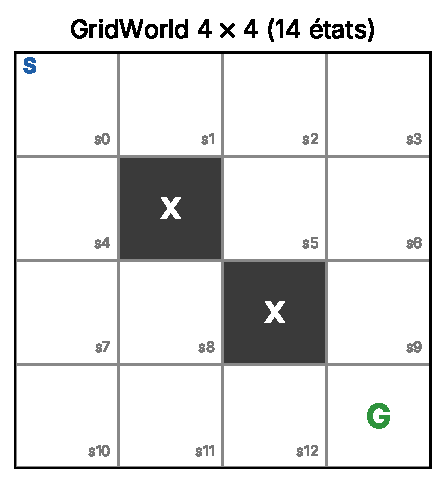
\includegraphics[width=0.85\linewidth]{fig1_gridworld.pdf}
\caption{Environnement : départ $S$, objectif $G$, obstacles $X$, numérotation des 14 états.}
\end{subfigure}\hfill
\begin{subfigure}[t]{0.52\linewidth}\centering
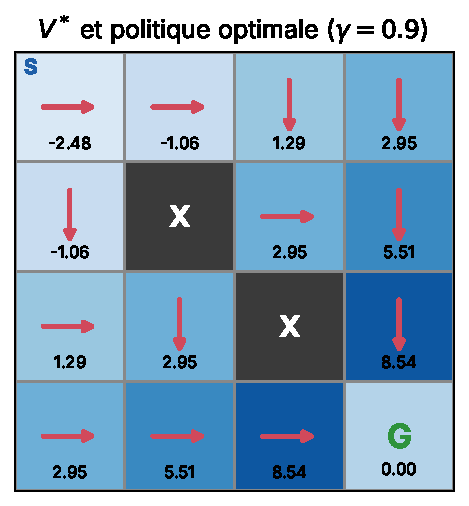
\includegraphics[width=0.75\linewidth]{fig2_optimal_policy.pdf}
\caption{$V^*(s)=\max_aQ^*(s,a)$ (valeur et couleur) et politique gloutonne pour $Q^*$, calculées par Value Iteration.}
\end{subfigure}
\caption{Figures 1 et 2 du cahier des charges : le GridWorld et sa politique optimale ($\gamma=0.9$).}
\label{fig-env}
\end{figure}

Le GridWorld est une grille $4\times4$ (\cref{fig-env}). Les deux obstacles ne sont pas des états : $\cS$ compte $14$ états, dont l'objectif $G$, absorbant. Les actions sont $\cA=\{\text{haut},\text{bas},\text{gauche},\text{droite}\}$. Pour que le problème soit réellement stochastique (et que le rôle du taux d'apprentissage soit visible), la dynamique est « glissante » : l'action demandée est exécutée avec probabilité $0.8$, et l'agent part dans chacune des deux directions perpendiculaires avec probabilité $0.1$. Si la direction réalisée mène hors de la grille ou dans un obstacle, l'agent reste sur place. Les récompenses sont
\[
R(s,a,s')=\begin{cases}+10&\text{si }s'=G,\\-5&\text{si }s'=s\ \text{(collision avec un bord ou un obstacle)},\\-1&\text{sinon (déplacement)},\end{cases}
\]
et $R(G,a,G)=0$. La pénalité de collision s'applique donc aussi aux bords, ce qui rend $R$ fonction de $(s,s')$ seulement et bien définie. On a $\Rmax=10$, donc $\abs{Q^*}\le\Rmax/(1-\gamma)=\ReturnBound$ d'après la \cref{prop-borne-retour} ; numériquement $\ninf{Q^*}=\QstarSup$, bien en dessous de cette borne de pire cas. Les épisodes partent de $S$ (sauf mention contraire) et s'arrêtent en $G$ ou après $200$ pas. Le code de l'environnement construit explicitement les tableaux $P[s,a,s']$ et $R[s,a,s']$ et vérifie que chaque $P(\cdot\mid s,a)$ est une loi de probabilité.

\FloatBarrier
\subsection{Value Iteration et vérification de la théorie}\label{sec-exp-vi}

\paragraph{Calcul de $Q^*$.} Avec $\gamma=0.9$, $Q_0=0$ et le critère d'arrêt $\ninf{Q_{k+1}-Q_k}<10^{-8}$, Value Iteration s'arrête après $\VIIters$ itérations, avec un dernier incrément $\VILastInc$. L'estimation a posteriori (\cref{thm-vi}) garantit alors $\ninf{Q_k-Q^*}\le\frac{\gamma}{1-\gamma}\times\VILastInc=\VIAPost$ ; l'erreur réelle, mesurée par rapport à une solution calculée avec une tolérance de $10^{-13}$, vaut $\VITrueErr$, ce qui respecte la garantie. Le \cref{tab-qstar} donne $Q^*$ et la \cref{fig-env} la politique optimale. On a $V^*(S)=\VstarS$.

\begin{table}[ht]
\centering
\small
\resizebox{\ifdim\width>\linewidth\linewidth\else\width\fi}{!}{\begin{tabular}{lrrrrr}
\toprule
case & haut & bas & gauche & droite & $V^*(s)$\\
\midrule
\TableQstar
\bottomrule
\end{tabular}}
\caption{Fonction $Q^*$ ($\gamma=0.9$) ; en gras les actions optimales. $Q^*(G,\cdot)=0$.}
\label{tab-qstar}
\end{table}

\paragraph{Lecture de la politique.} Le problème est symétrique par rapport à la diagonale (les obstacles sont sur la diagonale) : en $S$, « bas » et « droite » sont toutes deux optimales, avec la même valeur. Ailleurs l'action optimale est unique. La politique n'est pas un simple « plus court chemin » : en $(0,2)$ par exemple, aller vers le bas ($Q^*=1.291$) est préféré à aller vers le coin $(0,3)$ ($Q^*=1.103$). Les deux chemins ont la même longueur, mais les risques de collision dus au glissement diffèrent, et l'espérance dans $T$ en tient compte. Le plus petit écart d'action vaut $\Delta=\ActionGap$ (\cref{prop-perte}).

\begin{figure}[ht]
\centering
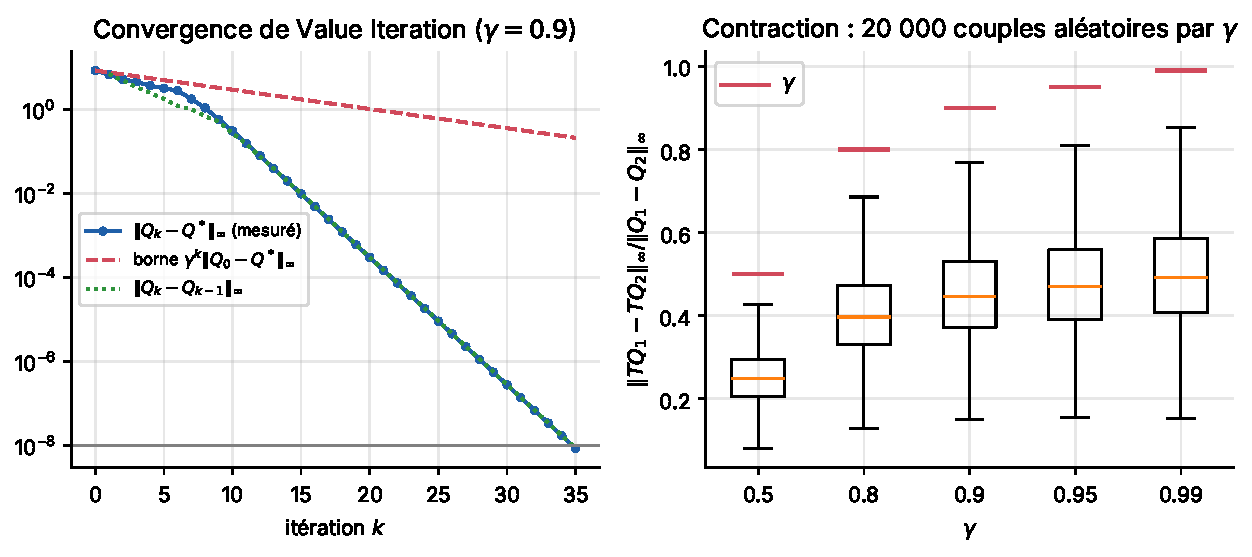
\includegraphics[width=\linewidth]{fig_vi_convergence_contraction.pdf}
\caption{À gauche : convergence de Value Iteration, comparée à la borne de Banach $\gamma^k\ninf{Q_0-Q^*}$. À droite : distribution du rapport $\ninf{TQ_1-TQ_2}/\ninf{Q_1-Q_2}$ pour $20\,000$ couples aléatoires et chaque $\gamma$ ; le trait rouge marque $\gamma$.}
\label{fig-vi}
\end{figure}

\paragraph{Vitesse de convergence.} La \cref{fig-vi} (gauche) montre que l'erreur reste toujours sous la borne $\gamma^k\ninf{Q_0-Q^*}$, comme le garantit le \cref{thm-vi}, mais qu'elle décroît beaucoup plus vite. La borne a priori $\gamma^k\ninf{Q_0-Q^*}\le10^{-8}$ demande $\VIBoundIters$ itérations ; il en a fallu $\VIIters$ pour que le critère d'arrêt soit atteint, avec une erreur réelle de $\VITrueErr$. Comme expliqué en \cref{sec-vi}, le rapport entre deux erreurs successives tend vers $\VIRatioLast$, qui coïncide avec $\gamma\rho=\AsymptoticRate$, où $\rho=\SpectralRho$ est le rayon spectral de $P_{\pi^*}$ restreinte aux états non terminaux.

\paragraph{Contraction.} La \cref{fig-vi} (droite) vérifie le \cref{thm-contraction} : pour chaque $\gamma$, aucun des $20\,000$ rapports n'a dépassé $\gamma$, et le cas d'égalité $Q_2=Q_1+c\1$ atteint exactement $\gamma$.

\paragraph{Politiques gloutonnes approchées.} Pour illustrer la \cref{prop-perte}, on a perturbé $Q^*$ par un bruit uniforme sur $[-\varepsilon,\varepsilon]$ ($2\,000$ tirages) et évalué exactement la politique gloutonne obtenue. Pour $\varepsilon=0.05<\Delta/2$, la perte maximale observée est $\LossEpsSmall$ : la politique reste optimale, comme prévu. Pour $\varepsilon=1$, la pire perte observée est $\LossEpsOne$, très en dessous de la borne $2\varepsilon/(1-\gamma)=\LossBoundOne$ ; pour $\varepsilon=2$, elle atteint $\LossEpsTwo$ (borne $\LossBoundTwo$). La borne est valide mais pessimiste.

\FloatBarrier
\subsection{Q-Learning : convergence de \texorpdfstring{$Q_t$}{Qt} vers \texorpdfstring{$Q^*$}{Q*}}\label{sec-exp-main}

\paragraph{Protocole.} $\gamma=0.9$, $\varepsilon=0.1$, $Q_0=0$, $\alpha_t=1/N_t(s,a)^{0.8}$ (qui vérifie Robbins-Monro), $100\,000$ épisodes, $\MainANSeeds$ graines. Toutes les $50$ épisodes on enregistre $E_t=\ninf{Q_t-Q^*}$ (sur les paires non terminales), l'erreur moyenne $\frac{1}{|\cS\setminus\{G\}||\cA|}\sum_{s,a}\abs{Q_t-Q^*}$, l'erreur à l'état de départ $\max_a\abs{Q_t(S,a)-Q^*(S,a)}$, la proportion d'états où l'action gloutonne est optimale, et la valeur exacte $V^{\pi_t}(S)$ de la politique gloutonne $\pi_t$. On compare deux réglages :
\begin{itemize}
\item \textbf{(A) départ fixe en $S$}, comme dans le cahier des charges ;
\item \textbf{(B) départs aléatoires} : chaque épisode part d'un état non terminal tiré uniformément. L'hypothèse de visite infinie est alors satisfaite de façon beaucoup plus homogène.
\end{itemize}

\begin{figure}[ht]
\centering
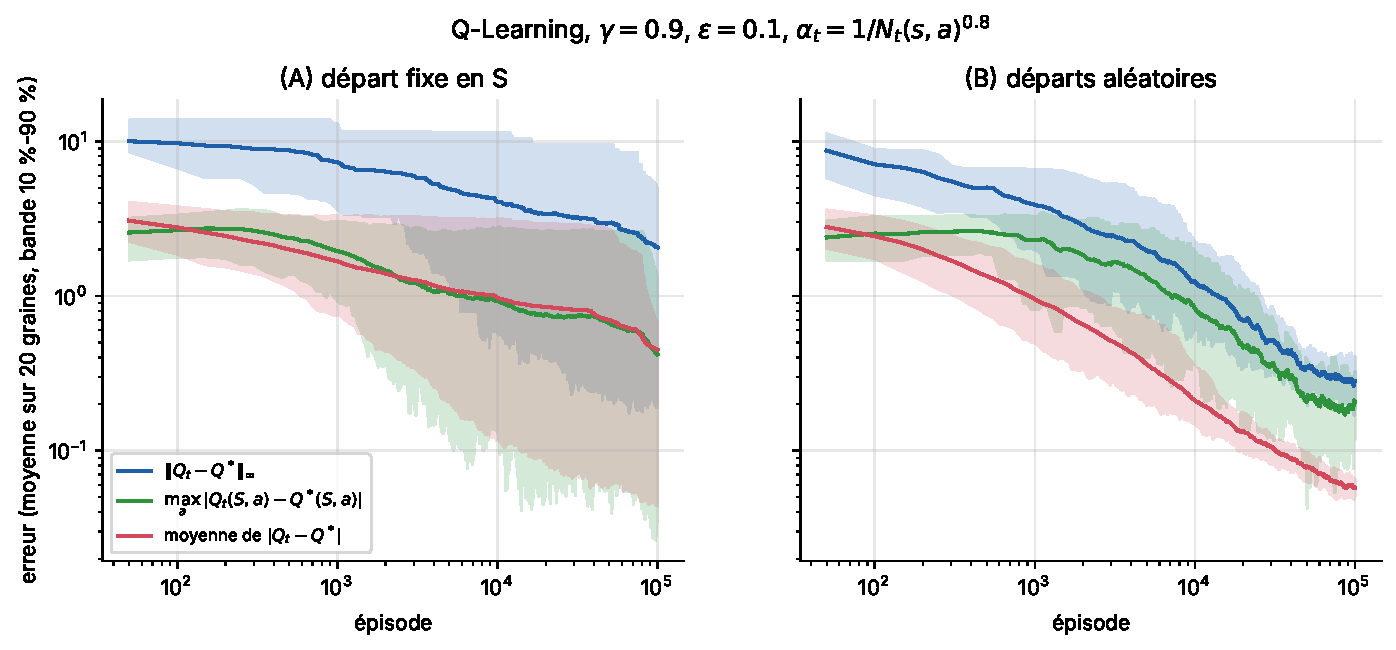
\includegraphics[width=\linewidth]{fig3_error_convergence.pdf}
\caption{Figure 3 du cahier des charges : $E_t=\ninf{Q_t-Q^*}$ en fonction du nombre d'épisodes (échelles logarithmiques), avec l'erreur moyenne et l'erreur à l'état de départ.}
\label{fig-main-error}
\end{figure}

\begin{table}[ht]
\centering
\small
\resizebox{\ifdim\width>\linewidth\linewidth\else\width\fi}{!}{\begin{tabular}{r|rrrr|rrrr}
\toprule
& \multicolumn{4}{c|}{(A) départ fixe} & \multicolumn{4}{c}{(B) départs aléatoires}\\
épisode & $E_t$ moy. & $E_t$ méd. & err. moy. & \% opt. & $E_t$ moy. & $E_t$ méd. & err. moy. & \% opt.\\
\midrule
\TableMain
\bottomrule
\end{tabular}}
\caption{Erreurs de Q-Learning ($20$ graines). « \% opt. » : proportion d'états non terminaux où l'action gloutonne pour $Q_t$ est optimale.}
\label{tab-main}
\end{table}

\paragraph{Résultat principal : on observe $Q_t\to Q^*$.} Dans le réglage (B), l'erreur uniforme décroît régulièrement de $\MainBErrHundred$ (épisode $100$) à $\MainBErrFinal$ (épisode $100\,000$), et l'erreur moyenne atteint $\MainBMeanErrFinal$ (\cref{fig-main-error}, \cref{tab-main}). Toutes les graines finissent avec une erreur comprise entre $\MainBErrMin$ et $\MainBErrMax$, et la politique gloutonne est optimale dans tous les états pour les $\MainBStab$ graines (médiane de l'épisode de stabilisation : $\MainBStabMedian$). C'est la confirmation expérimentale du \cref{thm-ql}. On remarque que l'erreur uniforme finale reste supérieure à $\Delta/2=\ActionGapHalf$ : la \cref{prop-perte} ne suffit donc pas à garantir l'optimalité de la politique gloutonne, qui est pourtant observée. La borne est un pire cas ; en pratique, l'erreur est concentrée sur des paires dont l'action n'est pas en compétition serrée avec l'action optimale.

\paragraph{Vitesse.} En coordonnées log-log, la pente de $E_t$ sur la fin de l'apprentissage vaut $\MainBSlope$ dans le réglage (B) : l'erreur décroît approximativement comme une puissance du nombre d'épisodes, beaucoup plus lentement que la décroissance géométrique de Value Iteration. C'est le prix de l'absence de modèle : il faut moyenner le bruit des transitions, et pour une moyenne empirique l'écart-type décroît en $n^{-1/2}$ (\cref{prop-rm-inv}).

\paragraph{Le rôle des visites : réglage (A).} Avec un départ toujours en $S$, l'erreur moyenne et l'erreur en $S$ décroissent bien ($\MainAMeanErrFinal$ et $\MainAStartErrFinal$ à la fin), mais l'erreur uniforme reste élevée en moyenne ($\MainAErrFinal$, médiane $\MainAErrFinalMedian$) avec une très grande dispersion entre graines (de $\MainAErrMin$ à $\MainAErrMax$). L'explication est donnée par le nombre de visites (\cref{fig-snapshots}) : la paire la moins visitée ne l'est en moyenne que $\MainAVisitsMin$ fois contre $\MainAVisitsMax$ pour la plus visitée, soit un rapport de $\MainAVisitsRatio$. Sur l'ensemble des paires et des graines, la corrélation entre $\log(N(s,a)+1)$ et $\log\abs{Q_t-Q^*}(s,a)$ vaut $\MainACorr$ : les paires peu visitées sont celles qui sont mal estimées. Dans $\MainAArgmaxFar$ graines sur $20$, le maximum de l'erreur se situe dans une case de bord éloignée de la trajectoire suivie ($(0,2)$, $(0,3)$, $(2,0)$ ou $(3,0)$).

\begin{figure}[ht]
\centering
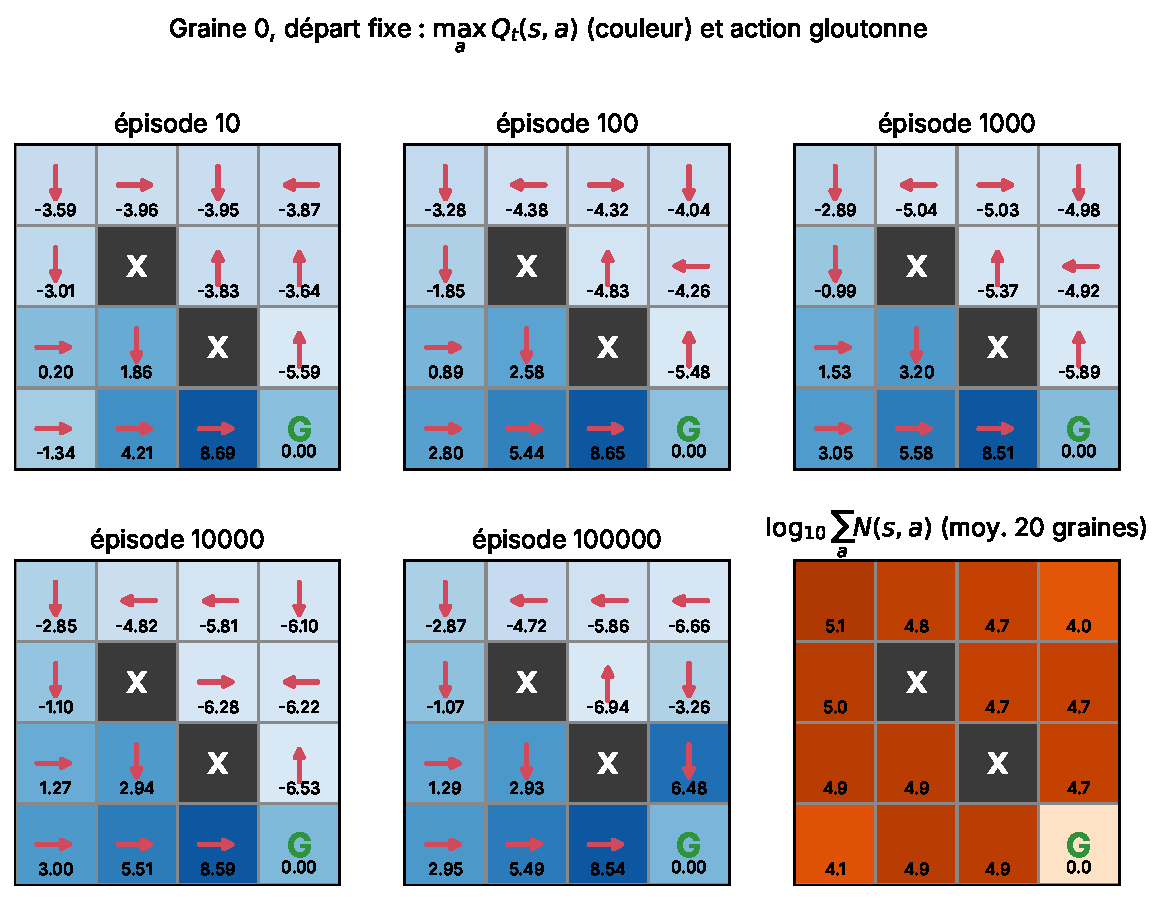
\includegraphics[width=0.92\linewidth]{fig_snapshots_visits.pdf}
\caption{Graine $0$, réglage (A) : $\max_aQ_t(s,a)$ et action gloutonne après $10$, $100$, $1\,000$, $10\,000$ et $100\,000$ épisodes ; dernier panneau : nombre de visites par état (en $\log_{10}$, moyenne sur 20 graines).}
\label{fig-snapshots}
\end{figure}

La \cref{fig-snapshots} montre un phénomène instructif. Comme « bas » et « droite » sont équivalentes en $S$, la graine $0$ s'est engagée sur le chemin passant par la colonne de gauche. Les cases de la partie droite de la grille sont alors rarement visitées, et la politique gloutonne y reste fausse même après $100\,000$ épisodes. Ce n'est pas une contradiction avec le \cref{thm-ql} : ces paires sont visitées infiniment souvent (grâce à $\varepsilon>0$ et au glissement), mais si rarement que la convergence, garantie à l'infini, n'est pas encore visible. Cette politique reste quasi optimale \emph{depuis $S$} : en moyenne $V^{\pi_t}(S)=\MainAGreedyValue$ contre $V^*(S)=\VstarS$, puisque les états mal estimés sont précisément ceux où l'agent ne va pas.

\begin{figure}[ht]
\centering
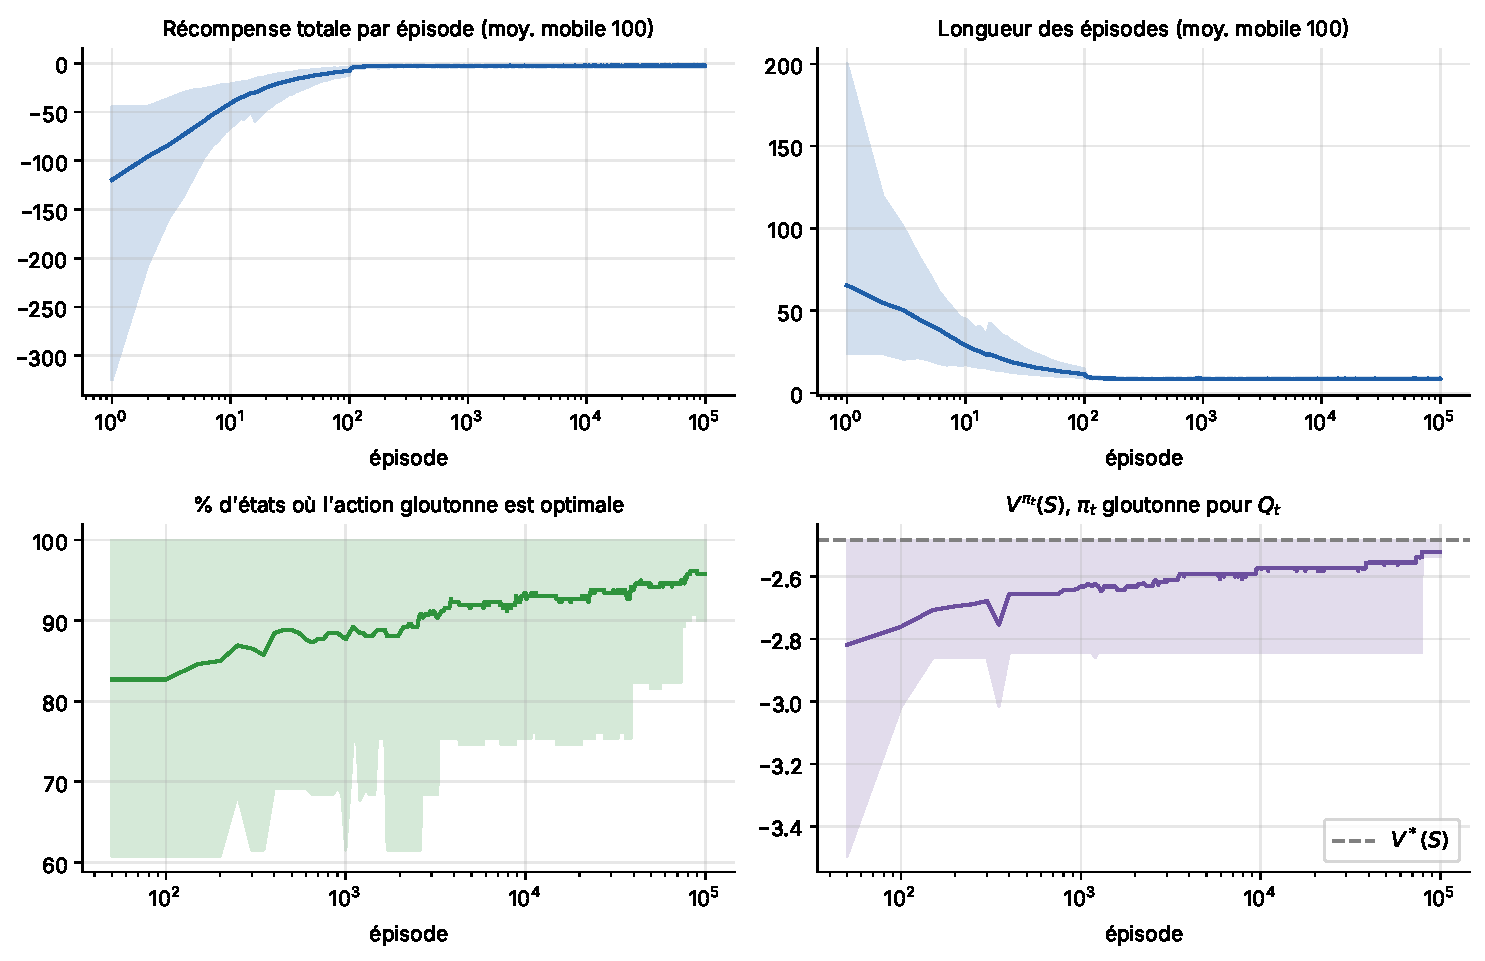
\includegraphics[width=0.95\linewidth]{fig4_reward_learning.pdf}
\caption{Figure 4 du cahier des charges, réglage (A) : récompense totale et longueur des épisodes pendant l'apprentissage (moyenne mobile sur 100 épisodes), proportion d'actions gloutonnes optimales, valeur exacte de la politique gloutonne depuis $S$.}
\label{fig-reward}
\end{figure}

\paragraph{Récompense et longueur des épisodes.} La \cref{fig-reward} montre l'apprentissage du point de vue de l'agent : la récompense par épisode augmente et la longueur des épisodes diminue jusqu'à se stabiliser (sur les $1\,000$ derniers épisodes : récompense moyenne $\MainAAvgReturn$, longueur moyenne $\MainAAvgLength$ pas). Ces grandeurs se stabilisent bien avant $E_t$ : la performance de l'agent dépend de la qualité de $Q$ sur les paires qu'il visite, pas sur toutes les paires. Elles incluent aussi le coût de l'exploration ($10\,\%$ d'actions aléatoires), si bien qu'elles restent inférieures à la performance de la politique gloutonne.

\FloatBarrier
\subsection{Influence de \texorpdfstring{$\gamma$}{gamma}}\label{sec-exp-gamma}

Protocole : réglage (B), $\varepsilon=0.1$, $\alpha_t=1/N_t^{0.8}$, $50\,000$ épisodes, $10$ graines ; pour chaque $\gamma$, $Q^*_\gamma$ est recalculé par Value Iteration. Comme $\ninf{Q^*_\gamma}$ dépend de $\gamma$, on compare des erreurs relatives $\ninf{Q_t-Q^*_\gamma}/\ninf{Q^*_\gamma}$.

\begin{table}[ht]
\centering
\small
\setlength{\tabcolsep}{4pt}
\resizebox{\ifdim\width>\linewidth\linewidth\else\width\fi}{!}{\begin{tabular}{rrrrrrrrrrr}
\toprule
$\gamma$ & $\frac{1}{1-\gamma}$ & VI (itér.) & borne & $\gamma\rho$ & $\ninf{Q^*_\gamma}$ & $V^*_\gamma(S)$ & $E_{1000}$ & $E_{50000}$ & relative & stab. (méd.)\\
\midrule
\TableGamma
\bottomrule
\end{tabular}}
\caption{Influence de $\gamma$. « VI » : itérations de Value Iteration pour $\ninf{Q_{k+1}-Q_k}<10^{-8}$ ; « borne » : plus petit $k$ tel que $\gamma^k\ninf{Q_0-Q^*_\gamma}\le10^{-8}$ (nombre d'itérations qui garantit a priori une erreur $10^{-8}$) ; $E_n$ : erreur $\ninf{Q_t-Q^*_\gamma}$ du Q-Learning après $n$ épisodes ; « relative » : $E_{50000}/\ninf{Q^*_\gamma}$ ; dernière colonne : médiane de l'épisode à partir duquel la politique gloutonne reste optimale.}
\label{tab-gamma}
\end{table}

\begin{figure}[ht]
\centering
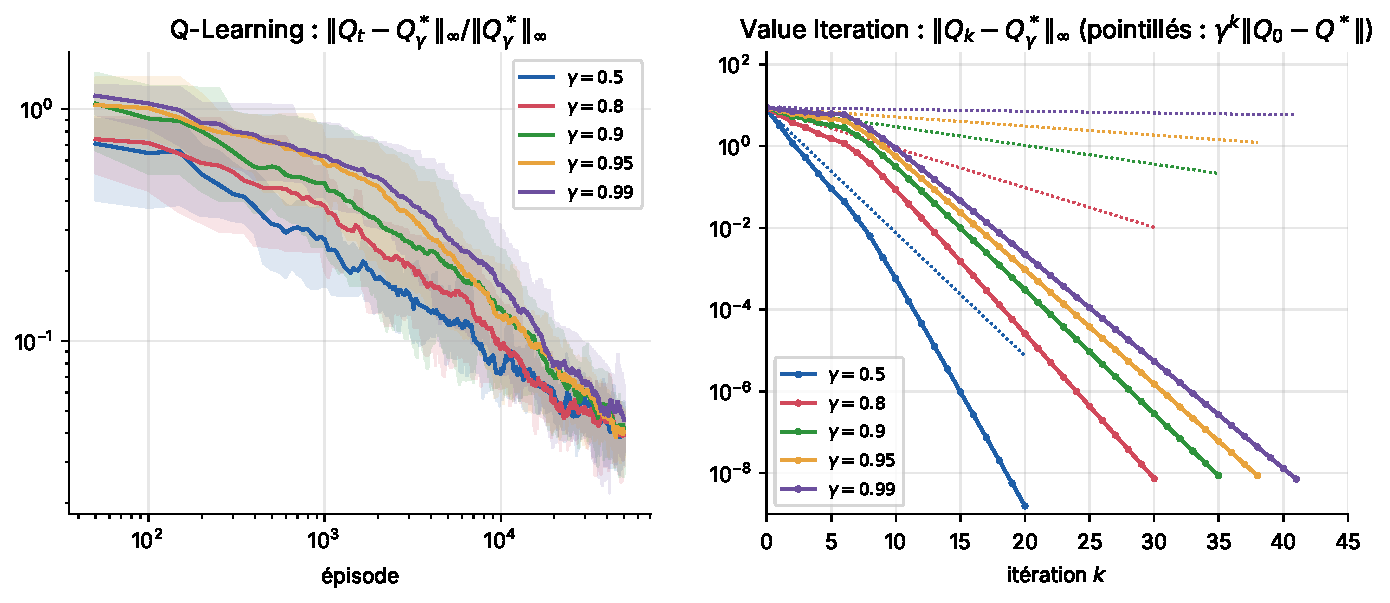
\includegraphics[width=\linewidth]{fig5_gamma.pdf}
\caption{Figure 5 du cahier des charges. À gauche : erreur relative du Q-Learning. À droite : Value Iteration pour chaque $\gamma$ (pointillés : borne $\gamma^k\ninf{Q_0-Q^*}$).}
\label{fig-gamma}
\end{figure}

\paragraph{Value Iteration.} La théorie prédit une convergence en $\gamma^k$ : le nombre d'itérations garanti par la borne explose quand $\gamma\to1$ (de $\GammaBoundLow$ pour $\gamma=0.5$ à $\GammaBoundHigh$ pour $\gamma=0.99$, \cref{tab-gamma}). Le nombre réel d'itérations augmente aussi, de $\GammaVIItersLow$ à $\GammaVIItersHigh$, mais beaucoup moins, parce que le taux effectif est $\gamma\rho$ et non $\gamma$ : l'absorption en $G$ borne l'horizon réel des trajectoires optimales, quel que soit $\gamma$.

\paragraph{Q-Learning.} Au début de l'apprentissage, l'erreur relative est d'autant plus grande que $\gamma$ est grand ($\GammaRelThousandLow$ pour $\gamma=0.5$ contre $\GammaRelThousandHigh$ pour $\gamma=0.99$ après $1\,000$ épisodes), et la politique se stabilise plus tôt pour les petits $\gamma$ (médiane $\GammaStabLow$ épisodes pour $\gamma=0.5$ contre $\GammaStabHigh$ pour $\gamma=0.95$ ; avec $\GammaStabHighest$ pour $\gamma=0.99$, la tendance n'est pas strictement monotone sur $10$ graines). Avec un $\gamma$ grand, la cible $r+\gamma\max Q(s',\cdot)$ dépend fortement d'estimations elles-mêmes encore fausses, et l'information sur la récompense finale doit se propager sur un horizon plus long. Après $50\,000$ épisodes, les erreurs relatives sont toutefois proches pour tous les $\gamma$ (entre $\GammaRelMin$ et $\GammaRelMax$) : dans ce petit environnement, l'effet de $\gamma$ sur la vitesse du Q-Learning reste modéré.

\paragraph{Politique obtenue.} Les ensembles d'actions optimales sont identiques pour les cinq valeurs de $\gamma$ testées (\cref{fig-gamma-pol}). C'est une propriété de cet environnement, pas un fait général : ici l'objectif est proche et toutes les politiques raisonnables l'atteignent en peu de pas. En revanche les valeurs changent. $V^*_\gamma(S)$ n'est pas monotone en $\gamma$ : pour $\gamma$ petit, la récompense $+10$, lointaine, est fortement actualisée ; pour $\gamma$ grand, elle compte davantage, mais les coûts de $-1$ par pas aussi. C'est l'effet « poids des récompenses futures » attendu.

\begin{figure}[ht]
\centering
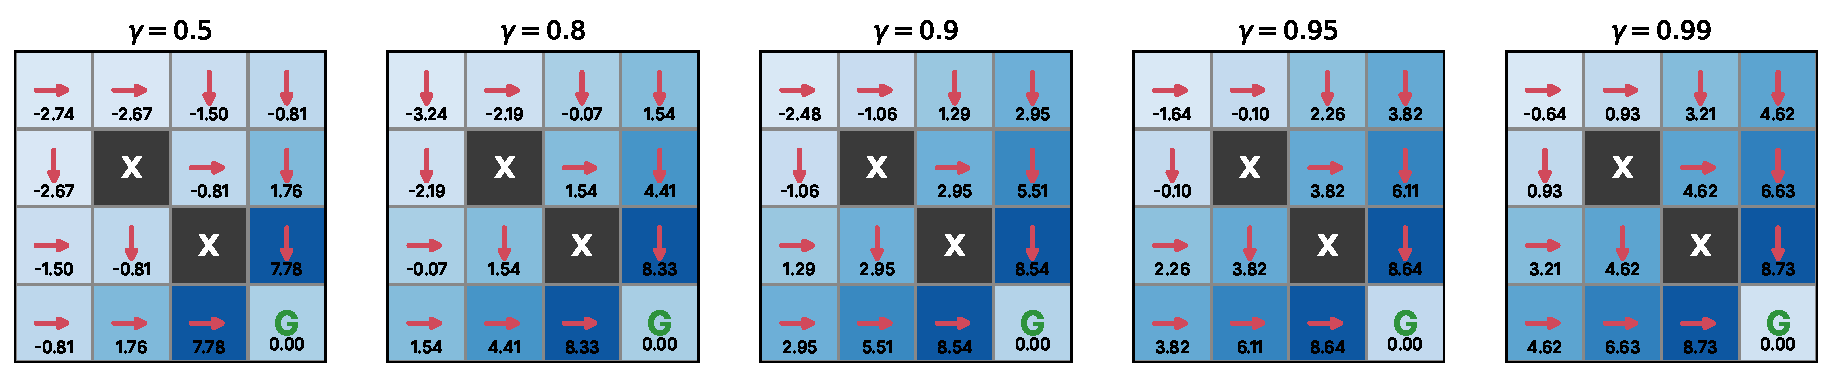
\includegraphics[width=\linewidth]{fig5b_gamma_policies.pdf}
\caption{$V^*_\gamma$ et une politique optimale pour chaque $\gamma$ (en $S$, les deux actions optimales sont équivalentes et l'affichage en choisit une).}
\label{fig-gamma-pol}
\end{figure}

\FloatBarrier
\subsection{Influence de \texorpdfstring{$\alpha$}{alpha}}\label{sec-exp-alpha}

\paragraph{Cas scalaire.} Avant le Q-Learning, on vérifie numériquement l'analyse de la \cref{sec-rm}. On estime la moyenne $m=\ScMean$ de la loi de la récompense obtenue en jouant « bas » en $(2,3)$ ($+10$, $-1$, $-5$ avec probabilités $0.8$, $0.1$, $0.1$ ; variance $\sigma^2=\ScVar$) par le schéma \eqref{eq-rm-scalaire}, avec $x_0=-20$, sur $\ScN$ pas et $\ScRuns$ répétitions.

\begin{table}[ht]
\centering
\small
\resizebox{\ifdim\width>\linewidth\linewidth\else\width\fi}{!}{\begin{tabular}{lrrrrr}
\toprule
pas $\alpha_n$ & $\sum_{n\le N}\alpha_n$ & $\sum_{n\le N}\alpha_n^2$ & $\E[(x_n-m)^2]$ final & moy. sur $n\ge10^4$ & théorie\\
\midrule
\TableScalar
\bottomrule
\end{tabular}}
\caption{Robbins-Monro scalaire ($N=\ScN$ pas, $\ScRuns$ répétitions ; les sommes sont partielles, jusqu'à $N$). Théorie : $\alpha\sigma^2/(2-\alpha)$ pour un pas constant (\cref{prop-rm-const}), $\sigma^2/n$ pour $1/n$ (\cref{prop-rm-inv}), convergence vers $0$ pour $1/n^{0.8}$ (\cref{thm-rm}).}
\label{tab-scalar}
\end{table}

Le \cref{tab-scalar} et la \cref{fig-alpha} (droite) confirment les trois propositions. Avec un pas constant, l'erreur quadratique se stabilise au niveau prédit $\alpha\sigma^2/(2-\alpha)$ : en moyenne sur la seconde moitié des pas, $\ScOneTail$ pour $\alpha=0.1$ (théorie $\ScTheoOne$) et $\ScFiveTail$ pour $\alpha=0.5$ (théorie $\ScTheoFive$). Avec $1/n$, elle vaut $\sigma^2/n$. Avec $1/n^2$ ($\sum\alpha_n<\infty$), l'estimateur se fige : comme $\alpha_1=1$, la condition initiale est effacée au premier pas, mais $x_n$ converge vers une moyenne pondérée d'un petit nombre d'observations, dont la variance ne tend pas vers $0$ ; c'est l'autre visage de la \cref{prop-rm-sommable} (la limite existe mais elle est aléatoire et différente de $m$).

\paragraph{Q-Learning.} Protocole : réglage (B), $\gamma=0.9$, $\varepsilon=0.1$, $50\,000$ épisodes, $10$ graines.

\begin{table}[ht]
\centering
\small
\resizebox{\ifdim\width>\linewidth\linewidth\else\width\fi}{!}{\begin{tabular}{lcrrrrrrr}
\toprule
pas & RM & $E_{1000}$ & $E_{10000}$ & $E_{50000}$ & err. moy. & fluct. & \% opt. & stab.\\
\midrule
\TableAlpha
\bottomrule
\end{tabular}}
\caption{Influence du taux d'apprentissage. « RM » : conditions de Robbins-Monro vérifiées ; $E_n=\ninf{Q_t-Q^*}$ après $n$ épisodes ; « fluct. » : écart-type de $E_t$ au cours du temps sur la seconde moitié de l'apprentissage (moyenne sur les graines) ; « stab. » : nombre de graines dont la politique gloutonne est optimale et stable à la fin.}
\label{tab-alpha}
\end{table}

\begin{figure}[ht]
\centering
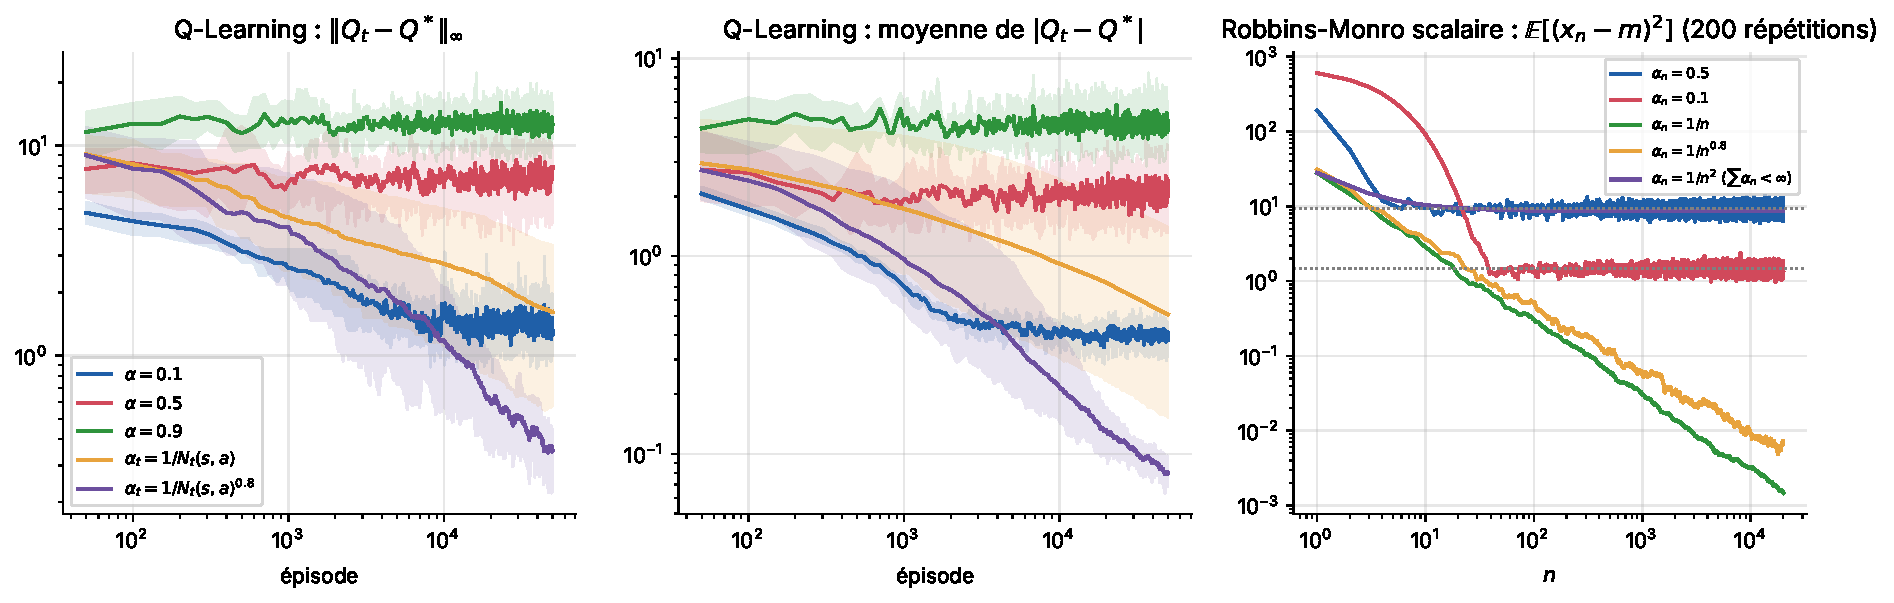
\includegraphics[width=\linewidth]{fig6_alpha.pdf}
\caption{Figure 6 du cahier des charges. Gauche et centre : erreurs du Q-Learning pour différents taux d'apprentissage. Droite : schéma de Robbins-Monro scalaire (pointillés : variances stationnaires théoriques $\alpha\sigma^2/(2-\alpha)$ pour $\alpha=0.1$ et $0.5$).}
\label{fig-alpha}
\end{figure}

Les résultats (\cref{tab-alpha}, \cref{fig-alpha}) reproduisent dans le Q-Learning ce que l'analyse scalaire prévoit.
\begin{itemize}
\item \textbf{Pas constants.} Aucun ne converge. Avec $\alpha=0.9$ ou $0.5$, $Q_t$ suit presque entièrement la dernière transition observée : l'erreur reste élevée ($\AlphaNineFinal$ et $\AlphaFiveFinal$ en fin d'apprentissage) et fluctue fortement (écart-type temporel $\AlphaNineStd$ et $\AlphaFiveStd$). Avec $\alpha=0.1$, l'erreur descend vite au début (c'est le meilleur réglage à $1\,000$ épisodes, $\AlphaOneThousand$), puis plafonne autour de $\AlphaOneFinal$, avec une fluctuation résiduelle : c'est le plancher de bruit de la \cref{prop-rm-const}.
\item \textbf{$\alpha_t=1/N_t(s,a)$.} Les conditions de Robbins-Monro sont satisfaites et les fluctuations sont faibles, mais la convergence est lente ($\AlphaInvFinal$ à $50\,000$ épisodes). Le pas $1/N$ fait de $Q_t(s,a)$ une moyenne de cibles calculées avec des estimations anciennes, très fausses au début ; leur poids ne décroît qu'en $1/N$. C'est le phénomène analysé par Even-Dar et Mansour (2003).
\item \textbf{$\alpha_t=1/N_t(s,a)^{0.8}$.} C'est le meilleur compromis : Robbins-Monro est satisfait, les anciennes cibles sont oubliées plus vite qu'avec $1/N$, et l'erreur atteint $\AlphaPolyFinal$ à $50\,000$ épisodes, avec la plus faible fluctuation ($\AlphaPolyStd$).
\end{itemize}
En résumé, la condition $\sum\alpha^2<\infty$ explique pourquoi les pas constants plafonnent, et la condition $\sum\alpha=\infty$ seule ne dit rien de la vitesse : deux suites qui vérifient Robbins-Monro peuvent avoir des comportements pratiques très différents.

\FloatBarrier
\subsection{Influence de \texorpdfstring{$\varepsilon$}{epsilon}}\label{sec-exp-eps}

Protocole : réglage (A) (départ fixe, de sorte que l'exploration ne vient que de la politique), $\gamma=0.9$, $\alpha_t=1/N_t^{0.8}$, $Q_0=0$, $50\,000$ épisodes, $10$ graines.

\begin{table}[ht]
\centering
\small
\setlength{\tabcolsep}{4pt}
\resizebox{\ifdim\width>\linewidth\linewidth\else\width\fi}{!}{\begin{tabular}{rrrrrrrrr}
\toprule
$\varepsilon$ & $E_{50000}$ & err. en $S$ & $V^{\pi_t}(S)$ & opt. depuis $S$ & \% opt. & récomp. moy. & paires jamais vues & visites min.\\
\midrule
\TableEps
\bottomrule
\end{tabular}}
\caption{Influence de $\varepsilon$ ($V^*(S)=\EpsVstar$). « opt.\ depuis $S$ » : nombre de graines dont la politique gloutonne finale a la valeur optimale en $S$ ; « récomp. moy. » : récompense moyenne par épisode \emph{pendant} l'apprentissage ; « paires jamais vues » et « visites min. » : moyennes sur les graines.}
\label{tab-eps}
\end{table}

\begin{figure}[ht]
\centering
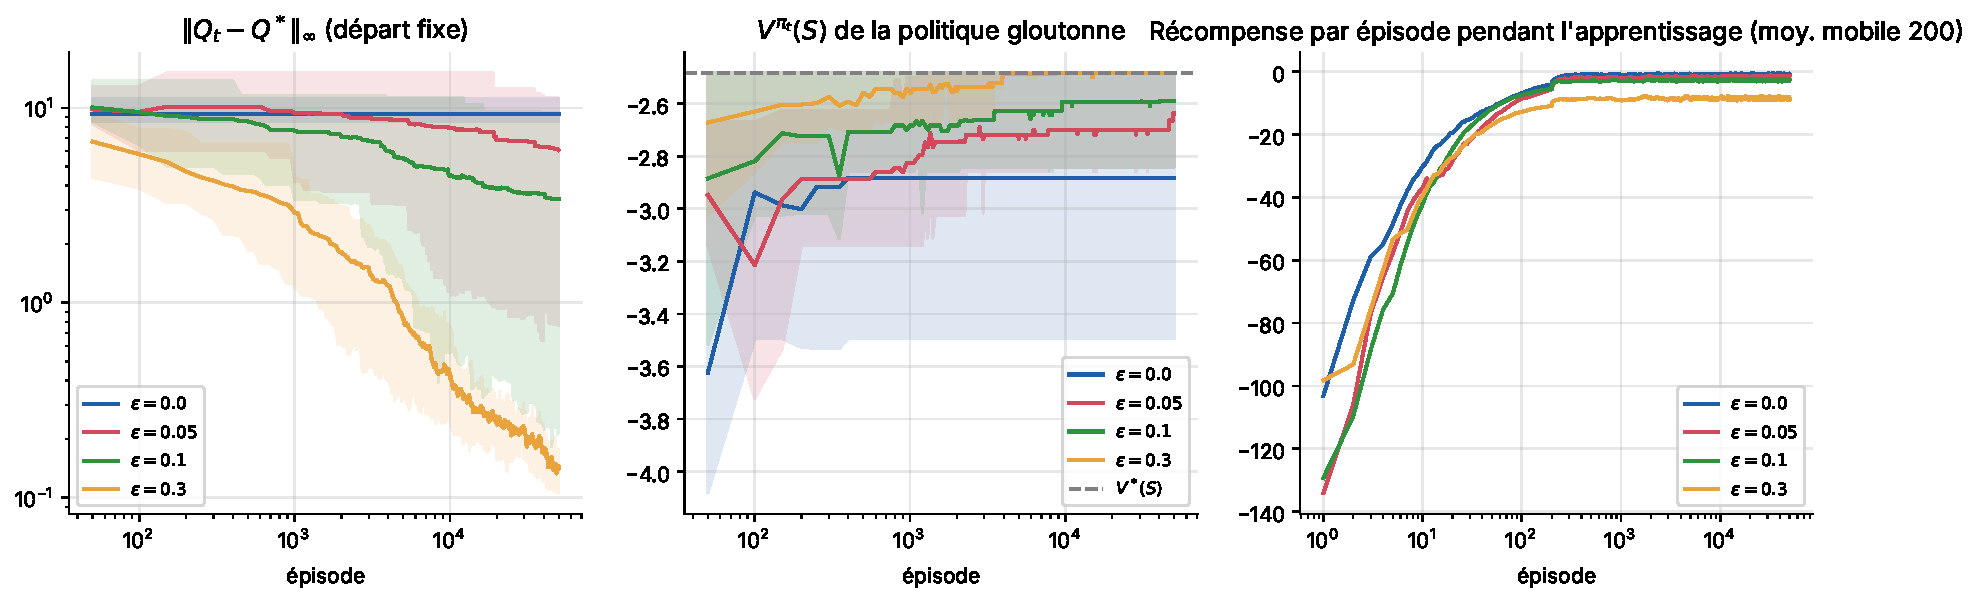
\includegraphics[width=\linewidth]{fig7_epsilon.pdf}
\caption{Figure 7 du cahier des charges : influence de $\varepsilon$ sur l'erreur, sur la valeur de la politique gloutonne et sur la récompense obtenue pendant l'apprentissage.}
\label{fig-eps}
\end{figure}

\paragraph{Sans exploration ($\varepsilon=0$), l'apprentissage se fige.} Avec $\varepsilon=0$, l'erreur $E_t$ vaut $\EpsZeroErrHundred$ dès l'épisode $100$ et n'évolue plus du tout ensuite ($\EpsZeroErr$ à $50\,000$ épisodes). En moyenne $\EpsZeroNever$ paires ne sont jamais visitées (jusqu'à $\EpsZeroNeverMax$ pour une graine) : pour elles $\sum_t\alpha_t(s,a)=0$, et le \cref{thm-ql} ne s'applique pas. Surtout, seules $\EpsZeroOptS$ graines sur $10$ trouvent une politique optimale depuis $S$ ; la pire atteint $V^{\pi}(S)=\EpsZeroValueMin$ contre $\VstarS$. C'est exactement le scénario de la \cref{sec-exploration} : l'agent exploite trop tôt une estimation incorrecte et ne découvre jamais les actions meilleures. Le phénomène se produit malgré l'initialisation optimiste $Q_0=0$ (\cref{rem-optimisme}), qui pousse à essayer chaque action au moins une fois dans les états visités, mais ne force ni à les réessayer, ni à visiter les autres états.

\paragraph{Plus d'exploration, meilleure estimation.} Quand $\varepsilon$ augmente, toutes les paires sont visitées, plus souvent (visites minimales moyennes : $\EpsFiveMinVisits$, $\EpsTenMinVisits$ puis $\EpsThirtyMinVisits$), et l'erreur finale diminue nettement : $\EpsFiveErr$, $\EpsTenErr$ puis $\EpsThirtyErr$. Avec $\varepsilon=0.3$, les $10$ graines trouvent la politique optimale depuis $S$ ($\EpsThirtyOptS/10$) et la politique gloutonne est optimale dans tous les états.

\paragraph{Le prix de l'exploration.} La récompense moyenne obtenue \emph{pendant} l'apprentissage évolue en sens inverse : $\EpsZeroReturn$ pour $\varepsilon=0$, $\EpsTenReturn$ pour $\varepsilon=0.1$, $\EpsThirtyReturn$ pour $\varepsilon=0.3$ (\cref{fig-eps}, droite). Explorer coûte, puisqu'une action sur $1/\varepsilon$ est aléatoire, alors qu'exploiter rapporte immédiatement mais empêche d'apprendre. C'est le compromis exploration contre exploitation, observé ici quantitativement : le meilleur $\varepsilon$ pour \emph{apprendre} $Q^*$ n'est pas le meilleur pour \emph{agir} pendant l'apprentissage. Une décroissance progressive de $\varepsilon_t$ permet de concilier les deux (\cref{sec-perspectives}).

\paragraph{Exploitation pure avec une initialisation pessimiste.} Pour isoler l'effet de l'exploration de celui de l'initialisation optimiste, on reprend l'expérience avec $Q_0=\PessQZero=-\Rmax/(1-\gamma)$, valeur inférieure à tout $Q^*(s,a)$, sur $\PessEpisodes$ épisodes (\cref{tab-pess}, \cref{fig-pess}).

\begin{table}[ht]
\centering
\small
\resizebox{\ifdim\width>\linewidth\linewidth\else\width\fi}{!}{\begin{tabular}{rrrrrrrr}
\toprule
$\varepsilon$ & $E_t$ final & $V^{\pi_t}(S)$ & opt. depuis $S$ & \% opt. & paires jamais vues & récomp. moy. & épisodes tronqués\\
\midrule
\TablePess
\bottomrule
\end{tabular}}
\caption{Initialisation pessimiste $Q_0=\PessQZero$, $\PessEpisodes$ épisodes, $10$ graines (« épisodes tronqués » : épisodes arrêtés à $200$ pas sans atteindre $G$, total sur les graines).}
\label{tab-pess}
\end{table}

\begin{figure}[ht]
\centering
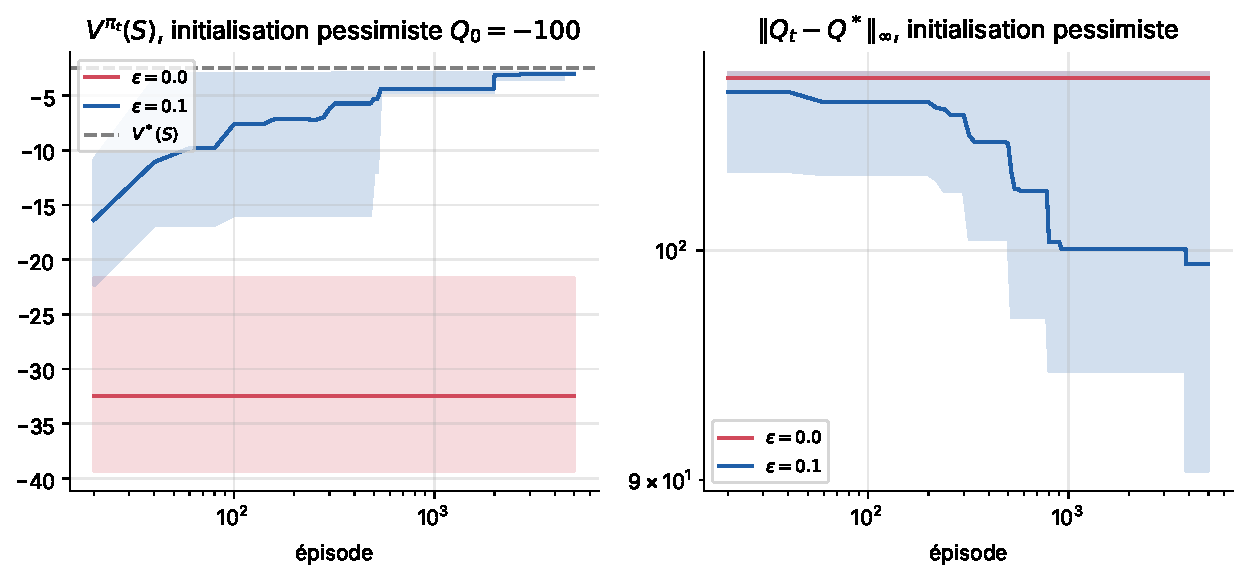
\includegraphics[width=0.85\linewidth]{fig7b_exploration_vs_exploitation.pdf}
\caption{Exploration contre exploitation avec une initialisation pessimiste : $\varepsilon=0$ reste bloqué, $\varepsilon=0.1$ progresse.}
\label{fig-pess}
\end{figure}

Avec $\varepsilon=0$, l'échec est complet. La première action essayée dans un état reçoit une valeur supérieure à $\PessQZero$ (par exemple, se cogner contre un mur mène vers $-5/(1-\gamma)=-50$), donc elle reste préférée à toutes les actions jamais essayées, qui gardent la valeur $\PessQZero$. L'agent tourne en rond : $\PessZeroTrunc$ épisodes sur $10\times\PessEpisodes$ sont tronqués à $200$ pas, la récompense moyenne par épisode vaut $\PessZeroReturn$, en moyenne $\PessZeroNever$ paires sur $52$ ne sont jamais visitées, et la politique gloutonne vaut en moyenne $V^{\pi_t}(S)=\PessZeroValue$ (contre $\VstarS$), sans aucune amélioration au cours du temps. Avec $\varepsilon=0.1$, la valeur de la politique gloutonne remonte à $\PessTenValue$ en $\PessEpisodes$ épisodes : l'exploration suffit à sortir de ces boucles, même si, sur cet horizon court, l'erreur uniforme reste dominée par les paires encore jamais visitées (en moyenne $\PessTenNever$), restées à leur valeur initiale. Cette expérience illustre directement la réponse attendue à la question du cahier des charges : un algorithme qui choisit toujours $\argmax_aQ(s,a)$ exploite une estimation incorrecte et peut ne jamais découvrir les actions meilleures.


%=====================================================================
\section{Discussion : théorie et expérience}\label{sec-discussion}
%=====================================================================

\paragraph{Ce que l'expérience confirme.}
\begin{itemize}
\item \emph{Contraction.} Le rapport $\ninf{TQ_1-TQ_2}/\ninf{Q_1-Q_2}$ ne dépasse jamais $\gamma$ et l'atteint dans le cas d'égalité prévu (\cref{thm-contraction}).
\item \emph{Point fixe et optimalité.} La politique gloutonne pour le point fixe calculé a pour fonction $Q$ ce point fixe lui-même, et aucune des $\NumRandomPolicies$ politiques aléatoires testées ne le dépasse (\cref{thm-optimalite}).
\item \emph{Value Iteration.} L'erreur reste sous la borne $\gamma^k\ninf{Q_0-Q^*}$ et le critère d'arrêt a posteriori est valide (\cref{thm-vi}).
\item \emph{Q-Learning.} Lorsque toutes les paires sont visitées régulièrement et que le pas vérifie Robbins-Monro, $\ninf{Q_t-Q^*}$ décroît vers $0$ et la politique gloutonne devient optimale pour toutes les graines (\cref{thm-ql}).
\item \emph{Hypothèses.} Chaque hypothèse du théorème a été « cassée » séparément, avec la conséquence prévue : pas constant $\Rightarrow$ plancher de bruit ; $\varepsilon=0$ $\Rightarrow$ paires jamais visitées, apprentissage figé et politique parfois sous-optimale.
\end{itemize}

\paragraph{Ce que la théorie ne dit pas et que l'expérience révèle.}
\begin{itemize}
\item \emph{La vitesse.} Le \cref{thm-ql} est asymptotique. En pratique, la convergence en norme infinie du Q-Learning est lente (décroissance approximativement polynomiale), alors que Value Iteration converge géométriquement, et même plus vite que $\gamma^k$ grâce à l'absorption ($\gamma\rho=\AsymptoticRate$).
\item \emph{La norme infinie est un critère sévère.} $\ninf{Q_t-Q^*}$ est dominée par la paire la plus mal estimée, qui est presque toujours la moins visitée. L'erreur moyenne, l'erreur en $S$ ou la valeur de la politique gloutonne convergent bien plus tôt. La norme infinie est la bonne norme pour la \emph{preuve} (c'est celle où $T$ est contractante), mais pas nécessairement la meilleure mesure de \emph{performance}.
\item \emph{« Infiniment souvent » n'est pas « souvent ».} Avec un départ fixe, l'hypothèse de visite infinie est satisfaite, mais certaines paires ne sont visitées que quelques centaines de fois en $100\,000$ épisodes. La symétrie du problème accentue l'effet : une graine qui s'engage sur un des deux chemins optimaux visite rarement l'autre côté de la grille.
\item \emph{Le choix du pas compte, même parmi les pas admissibles.} $1/N$ et $1/N^{0.8}$ vérifient tous deux Robbins-Monro, mais le second est nettement plus rapide, conformément à l'analyse d'Even-Dar et Mansour (2003).
\item \emph{L'initialisation compte.} $Q_0=0$ est optimiste dans ce problème et fournit une exploration implicite ; une initialisation pessimiste supprime ce mécanisme.
\end{itemize}

\paragraph{Limites de l'étude.} L'environnement est petit ($52$ paires état-action) et le modèle de glissement est simple ; les conclusions quantitatives (nombre d'épisodes, valeurs des erreurs) ne se transposent pas telles quelles à d'autres problèmes. Les balayages utilisent $10$ graines, ce qui suffit pour les tendances nettes mais pas pour départager des réglages proches (par exemple les épisodes de stabilisation pour $\gamma=0.95$ et $0.99$). Enfin, la preuve du lemme d'approximation stochastique n'a été qu'esquissée.

%=====================================================================
\section{Conclusion}
%=====================================================================

La convergence du Q-Learning repose sur une chaîne d'arguments dont chaque maillon a été établi ou expliqué :
\begin{enumerate}
\item la propriété de Markov permet d'écrire la valeur d'un état comme récompense immédiate plus valeur actualisée de l'état suivant (équations de Bellman) ;
\item l'opérateur d'optimalité $T$ est une contraction de rapport $\gamma$ en norme infinie, parce que le $\max$ et l'espérance ne dilatent pas les écarts et que seul le facteur $\gamma$ les modifie ;
\item le théorème de Banach donne alors un unique point fixe, qui est $Q^*$, et toute politique gloutonne pour $Q^*$ est optimale ; Value Iteration y converge géométriquement ;
\item le Q-Learning est une version stochastique, asynchrone et sans modèle de cette itération : sa cible est un estimateur sans biais de $(TQ_t)(s_t,a_t)$ ;
\item le bruit est éliminé par des pas qui vérifient $\sum\alpha=\infty$ (pour pouvoir apprendre) et $\sum\alpha^2<\infty$ (pour éteindre les fluctuations), à condition que chaque paire soit visitée infiniment souvent, ce que l'exploration $\varepsilon$-gloutonne garantit ;
\item sous ces hypothèses, $Q_t\to Q^*$ presque sûrement, et c'est la contraction de Bellman qui fournit la condition clé du lemme d'approximation stochastique.
\end{enumerate}
Les expériences sur un GridWorld stochastique confirment chacun de ces points et montrent leur portée : la convergence est observée quand les hypothèses sont satisfaites, et elle échoue de la manière prévue quand on les retire. Elles montrent aussi ce que la théorie asymptotique ne dit pas : la vitesse, très dépendante du pas, de l'exploration et de la fréquence des visites.

%=====================================================================
\section{Perspectives}\label{sec-perspectives}
%=====================================================================

\begin{itemize}
\item \textbf{Vitesses de convergence.} Des bornes non asymptotiques existent pour le Q-Learning (Even-Dar et Mansour, 2003, puis de nombreux travaux plus récents) ; les confronter aux courbes obtenues ici serait un prolongement naturel.
\item \textbf{Exploration décroissante.} Avec $\varepsilon_t\to0$ assez lentement (politiques GLIE), la politique de comportement elle-même devient optimale (Singh et al., 2000), ce qui résout le compromis observé en \cref{sec-exp-eps}.
\item \textbf{Biais de surestimation.} Le terme $\max_aQ_t(s',a)$ appliqué à des estimations bruitées est biaisé vers le haut ($\E[\max]\ge\max\E$) ; le Double Q-Learning (van Hasselt, 2010) corrige ce biais.
\item \textbf{SARSA et méthodes « on-policy ».} Remplacer $\max_aQ(s',a)$ par $Q(s',a')$, où $a'$ est l'action réellement jouée, donne SARSA, dont l'analyse fait intervenir l'opérateur $T^\pi$ plutôt que $T$.
\item \textbf{Approximation de fonctions.} Quand l'espace d'états est trop grand pour un tableau, on représente $Q$ par une fonction paramétrée (linéaire, puis réseau de neurones : Deep Q-Networks). La composition de $T$ avec une projection sur la classe de fonctions n'est plus contractante en norme infinie en général, et le Q-Learning peut diverger. Comprendre quand la contraction survit est une question de recherche active ; elle sort du périmètre de ce travail, mais les outils développés ici en sont le point de départ.
\end{itemize}

%=====================================================================
\begin{thebibliography}{99}
%=====================================================================
\bibitem{banach} S.~Banach. Sur les opérations dans les ensembles abstraits et leur application aux équations intégrales. \emph{Fundamenta Mathematicae}, 3:133--181, 1922.
\bibitem{bellman} R.~Bellman. \emph{Dynamic Programming}. Princeton University Press, 1957.
\bibitem{bertsekas} D.~P.~Bertsekas et J.~N.~Tsitsiklis. \emph{Neuro-Dynamic Programming}. Athena Scientific, 1996.
\bibitem{borkar} V.~S.~Borkar. \emph{Stochastic Approximation: A Dynamical Systems Viewpoint}. Cambridge University Press, 2008.
\bibitem{evendar} E.~Even-Dar et Y.~Mansour. Learning rates for Q-learning. \emph{Journal of Machine Learning Research}, 5:1--25, 2003.
\bibitem{jjs} T.~Jaakkola, M.~I.~Jordan et S.~P.~Singh. On the convergence of stochastic iterative dynamic programming algorithms. \emph{Neural Computation}, 6(6):1185--1201, 1994.
\bibitem{norris} J.~R.~Norris. \emph{Markov Chains}. Cambridge University Press, 1997.
\bibitem{puterman} M.~L.~Puterman. \emph{Markov Decision Processes: Discrete Stochastic Dynamic Programming}. Wiley, 1994.
\bibitem{rm} H.~Robbins et S.~Monro. A stochastic approximation method. \emph{The Annals of Mathematical Statistics}, 22(3):400--407, 1951.
\bibitem{singhyee} S.~P.~Singh et R.~C.~Yee. An upper bound on the loss from approximate optimal-value functions. \emph{Machine Learning}, 16(3):227--233, 1994.
\bibitem{glie} S.~Singh, T.~Jaakkola, M.~L.~Littman et C.~Szepesvári. Convergence results for single-step on-policy reinforcement-learning algorithms. \emph{Machine Learning}, 38(3):287--308, 2000.
\bibitem{sutton} R.~S.~Sutton et A.~G.~Barto. \emph{Reinforcement Learning: An Introduction}, 2\textsuperscript{e} édition. MIT Press, 2018.
\bibitem{szepes} C.~Szepesvári. \emph{Algorithms for Reinforcement Learning}. Morgan \& Claypool, 2010.
\bibitem{tsitsiklis} J.~N.~Tsitsiklis. Asynchronous stochastic approximation and Q-learning. \emph{Machine Learning}, 16(3):185--202, 1994.
\bibitem{vanhasselt} H.~van Hasselt. Double Q-learning. \emph{Advances in Neural Information Processing Systems}, 23, 2010.
\bibitem{watkins89} C.~J.~C.~H.~Watkins. \emph{Learning from Delayed Rewards}. Thèse de doctorat, University of Cambridge, 1989.
\bibitem{watkinsdayan} C.~J.~C.~H.~Watkins et P.~Dayan. Q-learning. \emph{Machine Learning}, 8(3--4):279--292, 1992.
\end{thebibliography}

\appendix

%=====================================================================
\section{Réponses courtes aux questions du cahier des charges}\label{sec-reponses}
%=====================================================================

Cette annexe sert d'aide-mémoire pour la soutenance ; chaque réponse renvoie à la partie qui la justifie.

\begin{enumerate}[leftmargin=*]
\item \textbf{Qu'est-ce qu'un MDP ?} Un quintuplet $(\cS,\cA,P,R,\gamma)$ : des états, des actions, un noyau de transition $P(s'\mid s,a)$, une récompense $R(s,a,s')$ et un facteur d'actualisation $\gamma<1$ (\cref{def-mdp}).
\item \textbf{Pourquoi est-il markovien ?} La loi de l'état suivant et de la récompense ne dépend du passé qu'à travers l'état et l'action présents, ce qui se lit dans la forme produit \eqref{eq-loi-traj} ; sous une politique fixée, les états forment une chaîne de Markov de matrice $P_\pi$ (\cref{prop-chaine-induite}).
\item \textbf{Qu'est-ce qu'une politique ?} Une règle de décision $\pi(a\mid s)$, loi sur les actions dans chaque état ; déterministe si elle choisit une action unique $\pi(s)$.
\item \textbf{Quelle différence entre $V$ et $Q$ ?} $V^\pi(s)$ est le retour moyen depuis $s$ en suivant $\pi$ ; $Q^\pi(s,a)$ impose la première action $a$. On a $V^\pi(s)=\sum_a\pi(a\mid s)Q^\pi(s,a)$. Connaître $Q$ permet d'agir ($\argmax_aQ$) sans connaître le modèle (\cref{sec-valeurs}).
\item \textbf{D'où vient Bellman ?} De la relation $G_t=R_{t+1}+\gamma G_{t+1}$, de la propriété de Markov (redémarrage, \cref{lem-redemarrage}) et de la formule des probabilités totales (\cref{thm-bellman-pi}).
\item \textbf{Pourquoi Bellman possède-t-il un point fixe ?} Parce que $T$ est une contraction de rapport $\gamma<1$ de l'espace complet $(\R^{\cS\times\cA},\ninf\cdot)$ et que le théorème de Banach s'applique (\cref{thm-contraction,thm-banach}).
\item \textbf{Pourquoi est-il unique ?} Si $Q_1$ et $Q_2$ sont fixes, $\ninf{Q_1-Q_2}=\ninf{TQ_1-TQ_2}\le\gamma\ninf{Q_1-Q_2}$, ce qui force $\ninf{Q_1-Q_2}=0$.
\item \textbf{Pourquoi Value Iteration converge-t-elle ?} C'est l'itération $Q_{k+1}=TQ_k$ du théorème de Banach : $\ninf{Q_k-Q^*}\le\gamma^k\ninf{Q_0-Q^*}$ (\cref{thm-vi}).
\item \textbf{Quelle différence entre Value Iteration et Q-Learning ?} Value Iteration calcule l'espérance exacte de $T$ avec le modèle et met à jour toutes les paires ; le Q-Learning remplace l'espérance par un échantillon, met à jour une seule paire par pas et moyenne le bruit avec un pas $\alpha_t$ (forme \eqref{eq-sa-form}).
\item \textbf{Pourquoi Q-Learning n'a-t-il pas besoin du modèle ?} Parce que sa cible $r_t+\gamma\max_aQ_t(s_{t+1},a)$ est un estimateur sans biais de $(TQ_t)(s_t,a_t)$ construit avec la seule transition observée (\cref{prop-td}) ; c'est la nature qui effectue le tirage selon $P$.
\item \textbf{Pourquoi faut-il explorer ?} Une paire visitée un nombre fini de fois n'est corrigée qu'un nombre fini de fois et ne peut pas converger ; un agent purement glouton peut se figer sur une estimation fausse (\cref{sec-exploration} ; observé avec $\varepsilon=0$, \cref{sec-exp-eps}).
\item \textbf{Rôle de $\gamma$ ?} Pondération du futur (horizon effectif $1/(1-\gamma)$), garantie de finitude des valeurs et rapport de contraction : plus $\gamma$ est proche de $1$, plus l'agent est prévoyant et plus la convergence garantie est lente.
\item \textbf{Rôle de $\alpha$ ?} Taille du pas de correction : compromis entre réactivité et stabilité. Robbins-Monro ($\sum\alpha=\infty$, $\sum\alpha^2<\infty$) garantit la convergence ; un pas constant laisse un plancher de bruit (\cref{sec-rm}, \cref{sec-exp-alpha}).
\item \textbf{Rôle de $\varepsilon$ ?} Fréquence des actions aléatoires : assure la visite de toutes les paires, au prix d'une moins bonne récompense pendant l'apprentissage (\cref{sec-exp-eps}).
\item \textbf{Sous quelles hypothèses Q-Learning converge-t-il ?} MDP fini, récompenses bornées, $\gamma<1$, chaque paire visitée infiniment souvent, pas vérifiant Robbins-Monro pour chaque paire ; alors $Q_t\to Q^*$ presque sûrement (\cref{thm-ql}).
\end{enumerate}

%=====================================================================
\section{Code et reproductibilité}\label{sec-code}
%=====================================================================

Le code est écrit en Python avec \texttt{numpy} et \texttt{matplotlib} uniquement, sans bibliothèque d'apprentissage par renforcement.

\begin{center}
\small
\begin{tabular}{l>{\raggedright\arraybackslash}p{0.58\linewidth}}
\toprule
fichier & contenu\\
\midrule
\texttt{src/environment.py} & GridWorld : états, actions, $P[s,a,s']$, $R[s,a,s']$, \texttt{reset()}, \texttt{step()}\\
\texttt{src/value\_iteration.py} & opérateurs $T$ et $T^\pi$, Value Iteration, évaluation exacte d'une politique\\
\texttt{src/q\_learning.py} & Q-Learning tabulaire, taux d'apprentissage, historique des mesures\\
\texttt{src/policies.py} & politiques gloutonne et $\varepsilon$-gloutonne\\
\texttt{src/markov\_chain.py} & chaînes de Markov : puissances, simulation, loi stationnaire\\
\texttt{src/utils.py} & norme infinie, sauvegardes, dessin de la grille et des politiques\\
\texttt{experiments/*.py} & une expérience par script (Markov, VI, principale, $\gamma$, $\alpha$, $\varepsilon$)\\
\texttt{tests/test\_core.py} & tests : noyau stochastique, lemme du max, contraction, point fixe, bornes\\
\texttt{report/make\_results.py} & génération des nombres et tableaux du rapport à partir des données\\
\bottomrule
\end{tabular}
\end{center}

Pour tout reproduire : \texttt{pip install -r requirements.txt}, puis \texttt{python run\_all.py} (environ quinze minutes sur deux cœurs), puis \texttt{python report/make\_results.py} et la compilation de \texttt{report/report.tex}. Chaque expérience fixe ses graines (\texttt{numpy.random.default\_rng(seed)}, flux séparés pour l'agent et l'environnement), si bien que deux exécutions donnent des résultats identiques.


\end{document}
